\chapter{Documento dei requisiti software}

\section{Obiettivi della Raccolta dei Requisiti}
% Descrizione: Spiega l'importanza della raccolta dei requisiti e come è stata condotta (interviste, workshop, analisi documentale).
% Stakeholder Coinvolti: Elenca gli stakeholder chiave e il loro ruolo nella definizione dei requisiti.
La raccolta dei requisiti è una fase fondamentale per garantire che il prodotto finale soddisfi gli stakeholder e gli obiettivi prefissati.

L'obiettivo principale di questa fase è identificare, analizzare e documentare le esigenze e le aspettative delle parti interessate, in particolare sono stati individuati tre tipi di requisiti: funzionali, non funzionali e di dominio.
\begin{itemize}
	\item I requisiti funzionali definiscono le funzionalità che il sistema deve offrire, descrivendo come il software interagirà con gli utenti e con altri sistemi.
	\item I requisiti non funzionali, riguardano le qualità del sistema, come le prestazioni, la sicurezza, l'usabilità e la scalabilità.
	\item I requisiti di dominio definiscono le regole di comportamento che il sistema deve applicare.
\end{itemize}

\newpage

\section{Requisiti individuati}
\subsection{Requisiti funzionali}
\begin{itemize}
	\item l'utente può registrare un nuovo account
	\item l'utente può utilizzare un'account da lui registrato per accedere al sistema
	\item l'utente può registrarsi utilizando credenziali di terze pari (es.: google, facebook, …)
	\item l'utente può personalizzare il proprio profilo (non obbligatorio):
	      \begin{itemize}[label={\tiny$\blacksquare$}]
		      \renewcommand{\labelitemi}{\tiny$\blacksquare$}
		      \item aggiungere nome e cognome
		      \item aggiungere una breve bio
		      \item link al proprio sito web
		      \item link ai propri social
	      \end{itemize}
	      \medskip
	\item l'utente può creare un'asta
	      \begin{itemize}[label={\tiny$\blacksquare$}]
		      \item inserisce la foto
		      \item inserisce la descrizione
		      \item inserisce la categoria
		      \item asta all'inglese
		            \begin{itemize}[label={\tiny$-$}]
			            \item il venditore inserisce una base d'asta (visibile a tutti)
			            \item ***(dubbio colloquio 3)*** L'asta include un intervallo di tempo fisso per presentare nuove offerte (di default 1 ora)
			            \item ***(dubbio colloquio 3)*** L'asta include una soglia di rialzo (di default 10€)
		            \end{itemize}
		      \item l'utente può creare un asta al ribasso e inserisce:
		            \begin{itemize}[label={\tiny$-$}]
			            \item un prezzo iniziale
			            \item la durata del timer per il decremento del prezzo (di default 1 ora).
			            \item l'importo per ciascun decremento
			            \item il prezzo minimo segreto (non visibili pubblicamente).
		            \end{itemize}
		      \item l'utente può creare un asta silenziosa
		            \begin{itemize}[label={\tiny$-$}]
			            \item inserisce data e ora di scadenza
			            \item può accettare un'offerta
		            \end{itemize}
	      \end{itemize}

	      \medskip
	\item l'utente può presentare un'offerta (per qualsiasi tipo d'asta) \medskip

	\item l'utente può cercare un'asta per parola chiave
	\item l'utente può filtrare le aste per categoria (tecnologia, giocattoli, …) \medskip

	\item l'utente può visualizzare i dettagli di un'asta
	\item l'utente può visualizzare il profilo del venditore dell'asta \medskip

	\item Visualizzazione storico aste create (in corso e concluse)
	\item Visualizzazione storico a cui hai partecipato (in corso e concluse)
\end{itemize}

\newpage
\subsection{Requisiti non funzionali}
\begin{itemize}
	\item il sistema deve gestire la concorrenza in caso di offerte uguali contemporaneamente:

	      Se, in un'asta all'inglese, più compratori fanno la stessa offerta contemporaneamente, solo uno avrà la meglio.

	      Stesso discorso per un'asta al ribasso, se più compratori decidono di acquistare l'asta a quel prezzo, solo uno avrà la meglio.
\end{itemize}
\begin{enumerate}
	\item {\sffamily \textbf{Usabilità}}:\\
	      L'interfaccia utente deve essere intuitiva e facile da utilizzare, con una chiara visualizzazione delle informazioni relative alle aste e ai profili utenti.

	\item {\sffamily \textbf{Performance}}:\\
	      Il sistema deve gestire in modo efficiente un grande numero di aste e utenti, garantendo tempi di risposta rapidi, specialmente durante la presentazione delle offerte e la gestione dei timer.

	\item {\sffamily \textbf{Scalabilità}}:\\
	      Il sistema deve essere scalabile per supportare un numero crescente di utenti, aste e operazioni contemporanee senza compromettere le prestazioni.

	\item {\sffamily \textbf{Sicurezza}}:\\
	      Gli utenti devono poter registrarsi e autenticarsi in modo sicuro, anche tramite provider di terze parti.

	      Devono essere implementate misure per proteggere le offerte e i dati personali degli utenti.

	\item {\sffamily \textbf{Affidabilità}}:\\
	      Il sistema deve essere altamente disponibile, minimizzando i tempi di inattività.

	      I dati relativi alle aste, alle offerte e ai profili devono essere conservati in modo sicuro e accessibili in qualsiasi momento.
\end{enumerate}

\newpage
\subsection{Requisiti di dominio}
\begin{itemize}
	\item l'email è univoca per ogni account. Non possono esserci più account con una sola mail
	\item un account è sia venditore che compratore
	\item l'utente non può acquistare le aste create da lui stesso
	\item l'asta può essere di diversi tipi: all'inglese, al ribasso, silenziosa:
	      \begin{itemize}[label={\tiny$\blacksquare$}]
		      \item {\sffamily \textbf{Asta all'inglese}}: Un formato in cui le offerte incrementano il prezzo fino alla scadenza del timer, con vincita al miglior offerente.
		      \item {\sffamily \textbf{Asta al ribasso}}: Un formato in cui il prezzo diminuisce con il tempo, e la vendita avviene al primo offerente che accetta il prezzo corrente.
		      \item {\sffamily \textbf{Asta silenziosa}}: Un formato in cui le offerte sono segrete e il venditore sceglie una sola offerta da accettare.
	      \end{itemize}
	\item asta all'inglese:
	      \begin{itemize}[label={\tiny$\blacksquare$}]
		      \item l'offerta può essere presentata a partire dal prezzo corrente.

		            se è la prima offerta può offrire il prezzo base, altrimenti deve presentare un'offerta più alta rispetto al prezzo corrente.

		            Il rialzo dev'essere un multiplo della soglia impostata nell'offerta ***(dubbio colloquio, dev'essere di X alla volta o anche multipli di X?)***

		      \item quando viene presentata un'offerta, il timer viene resettato e il prezzo corrente viene aggiornato
		      \item allo scadere del timer:
		            \begin{itemize}[label={\tiny$-$}]
			            \item l'asta si conclude
			            \item vince l'ultima offerta fatta
			            \item il venditore e gli acquirenti che hanno partecipato all'asta visualizzano una notifica.
		            \end{itemize}
	      \end{itemize}
	\item asta al ribasso:
	      \begin{itemize}[label={\tiny$\blacksquare$}]
		      \item al raggiungimento del timer, il prezzo verrà decrementato dell'importo previsto e il timer riparte
		      \item il prodotto è venduto al primo acquirente che presenta un'offerta
		      \item Se il prezzo raggiunge il prezzo minimo segreto senza offerte, l'asta fallisce e il venditore riceve una notifica. ***(dubbio colloquio l'offerta fallisce al raggiungimento del prezzo minimo oppure fallisce al ribasso successivo al prezzo minimo?)***
	      \end{itemize}
	\item asta silenziosa:
	      \begin{itemize}[label={\tiny$\blacksquare$}]
		      \item le offerte degli utenti sono segrete, non visibili agli altri utenti ma solo al venditore
		      \item il venditore può accettare una sola offerta
		      \item quando il venditore accetta un'offerta, viene inviata una notifica all'acquirente.
	      \end{itemize}

\end{itemize}

\newpage

\section{Modello dei casi d'uso}
\subsection{Tabella}

{
	\setlength{\tabcolsep}{10pt} % Padding orizzontale
	\renewcommand{\arraystretch}{1.5} % Padding verticale

	\begin{tabular}{|l|p{330pt}|}
		\hline
		\textbf{Attore}    & \textbf{Casi d'uso}                                        \\ \hline
		Utente non loggato & \begin{itemize}[leftmargin=15pt]
			                     \setlength{\itemsep}{0pt}  % Riduce lo spazio tra gli elementi della lista
			                     \setlength{\parskip}{0pt}  % Riduce lo spazio tra i paragrafi
			                     \item registrazione con email
			                     \item registrazione con credenziali di terze parti (Google)
			                     \item Accesso al sistema
		                     \end{itemize} \\ \hline
		\makecell{Utente non loggato                                                    \\ (venditore/acquirente)} &
		\begin{itemize}[leftmargin=15pt]
			\setlength{\itemsep}{0pt}  % Riduce lo spazio tra gli elementi della lista
			\setlength{\parskip}{0pt}  % Riduce lo spazio tra i paragrafi
			\item Personalizza il profilo
			\item Visualizza storico
			      \begin{itemize}
				      \item aste create (in corso e concluse)
				      \item a cui hai partecipato (in corso e concluse)
			      \end{itemize}
			\item Ricerca asta per parola chiave
			\item Filtra asta per categoria
			\item Visualizza dettagli di un'asta
			\item Visualizza il profilo del venditore

		\end{itemize}\medskip

		\begin{itemize}[leftmargin=15pt]
			\setlength{\itemsep}{0pt}  % Riduce lo spazio tra gli elementi della lista
			\setlength{\parskip}{0pt}  % Riduce lo spazio tra i paragrafi
			\item Crea asta all'inglese
			\item Crea asta al ribasso
			\item Crea asta silenziosa
		\end{itemize}\medskip

		\begin{itemize}[leftmargin=15pt]
			\setlength{\itemsep}{0pt}  % Riduce lo spazio tra gli elementi della lista
			\setlength{\parskip}{0pt}  % Riduce lo spazio tra i paragrafi
			\item Piazza un'offerta per l'asta all'inglese
			\item Piazza un'offerta per l'asta al ribasso
			\item Piazza un'offerta per l'asta silenziosa
		\end{itemize}\medskip

		\begin{itemize}[leftmargin=15pt]
			\item Accetta un'offerta di un'asta silenziosa
		\end{itemize}
		\\ \hline
	\end{tabular}
}

\subsection{Descrizioni dettagliate}
\begin{itemize}
	\item \textbf{Registrazione con email.}\\
	      L'utente che desidera registrarsi, può farlo inserendo dati quali: email, nome, cognome e password. I dati inseriti sono soggetti a verifica da parte del sistema (ad esempio: la mail deve essere in un formato valido).

	      Una volta effettuata la registrazione, se questa ha avuto successo, l'utente accede al sistema.

	\item \textbf{Registrazione con credenziali di terze parti (Google).}\\
	      L'utente può registrarsi più utilizzando il proprio account Google. Una volta effettuata la registrazione, se questa ha avuto successo, l'utente accede al sistema.

	\item \textbf{Accesso al sistema.}\\
	      L'utente che ha già effettuato la registrazione in precedenza può accedere al sistema utilizzando la mail con la quale si è registrato e la propria password.

	\item \textbf{Personalizzazione del profilo.}\\
	      Andando nella sezione “Profilo”, l'utente può visualizzare le proprie informazioni e modificarle. Può aggiungere informazioni quali: bio, link al proprio sito personale, link ai social ed area geografica.

	\item \textbf{Visualizzazione storico aste create (in corso e concluse).}\\
	      Andando nella sezione “Storico Aste”, l'utente può visualizzare sia le aste a cui ha preso parte (quelle in corso per cui ha piazzato un'offerta, e quelle concluse) sia le aste che ha creato (in corso e concluse).

	\item \textbf{Ricerca aste per parola chiave.}\\
	      Nella homepage l'utente può selezionare la barra di ricerca e inserire delle parole chiave per filtrare le aste per descrizione, in modo da trovare più velocemente ciò a cui è interessato.

	      \textit{Nota: Se anche il filtraggio per categoria è attivato, la ricerca viene raffinata ulteriormente (parola chiave + categoria).}

	\item \textbf{Filtraggio aste per categoria.}\\
	      Nella homepage l'utente può selezionare dei pulsanti per filtrare le aste visualizzate per categoria.

	\item \textbf{Visualizza dettagli di un'asta.}\\
	      L'utente interessato ad un'asta può cliccarla per accedere alla pagina di dettaglio e visualizzare tutte le informazioni di cui ha bisogno. Da questa schermata è anche possibile fare un'offerta (se l'asta è ancora in corso) e visualizzare il profilo del venditore.

	\item \textbf{Visualizza il profilo del venditore.}\\
	      L'utente che sta visualizzando un'asta può cliccare sul nome del venditore per visualizzare la pagina profilo del venditore.

	\item \textbf{Creare asta all'inglese.}\\
	      Dalla schermata home, l'utente clicca sul pulsante “Crea Asta”, poi clicca sul pulsante "Asta all'inglese". Viene visualizzata una nuova schermata in cui deve inserire tutte le informazioni necessarie tra cui: immagine, descrizione, categoria, base d'asta, soglia di rialzo e il timer.

	\item \textbf{Creare asta al ribasso.}\\
	      Dalla schermata home, l'utente clicca sul pulsante “Crea Asta”, poi clicca sul pulsante "Asta al ribasso". Viene visualizzata una nuova schermata in cui deve inserire tutte le informazioni necessarie tra cui: immagine, descrizione, categoria, prezzo iniziale, prezzo minimo, importo di cui decrementare, timer prima di un decremento.

	\item \textbf{Creare asta silenziosa.}\\
	      Dalla schermata home, l'utente clicca sul pulsante “Crea Asta”, poi clicca sul pulsante "Asta silenziosa". Viene visualizzata una nuova schermata in cui deve inserire tutte le informazioni necessarie tra cui: immagine, descrizione, categoria, scadenza.

	\item \textbf{Piazzare un'offerta per l'asta all'inglese.}\\
	      L'utente che si trova sulla schermata di un'asta all'inglese inserisce l'importo dell'offerta che vuole piazzare, poi clicca sul pulsante "conferma offerta".

	\item \textbf{Piazzare un'offerta per l'asta al ribasso.}\\
	      L'utente che si trova sulla schermata di un'asta al ribasso può cliccare il pulsante “Acquista” ed aggiudicarsi automaticamente l'asta. Dopo quest'operazione il sistema mostra una notifica che informa l'utente dell'esito dell'asta.

	\item \textbf{Piazzare un'offerta per l'asta silenziosa.}\\
	      L'utente che si trova sulla schermata di un'asta silenziosa può inserire un'offerta e cliccare sul pulsante "conferma offerta" per inviare l'offerta.

	\item \textbf{Accetta un'offerta di un'asta silenziosa.}\\
	      L'utente che ha creato un'asta silenziosa, può andare nello storico delle aste create, selezionare un'asta in corso e accettare un'offerta.

\end{itemize}

\newpage
\subsection{Diagrammi}
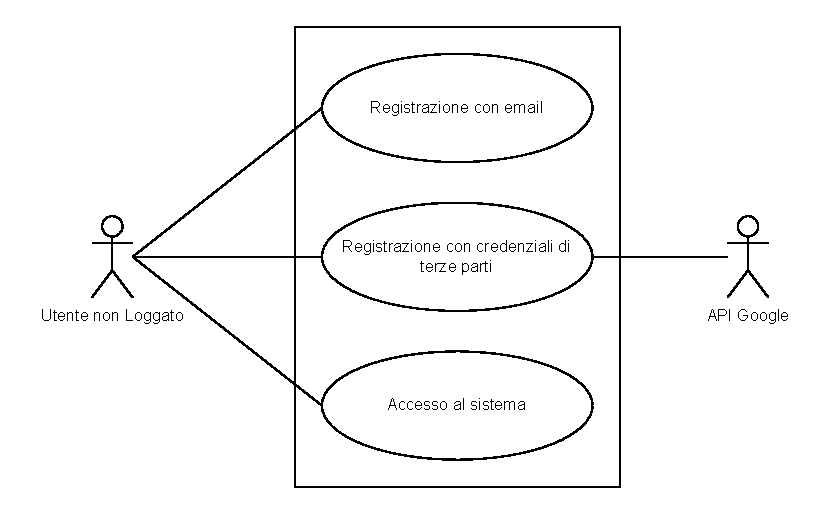
\includegraphics[width=.7\textwidth]{assets/utente_non_loggato_use_case_diagram.pdf}

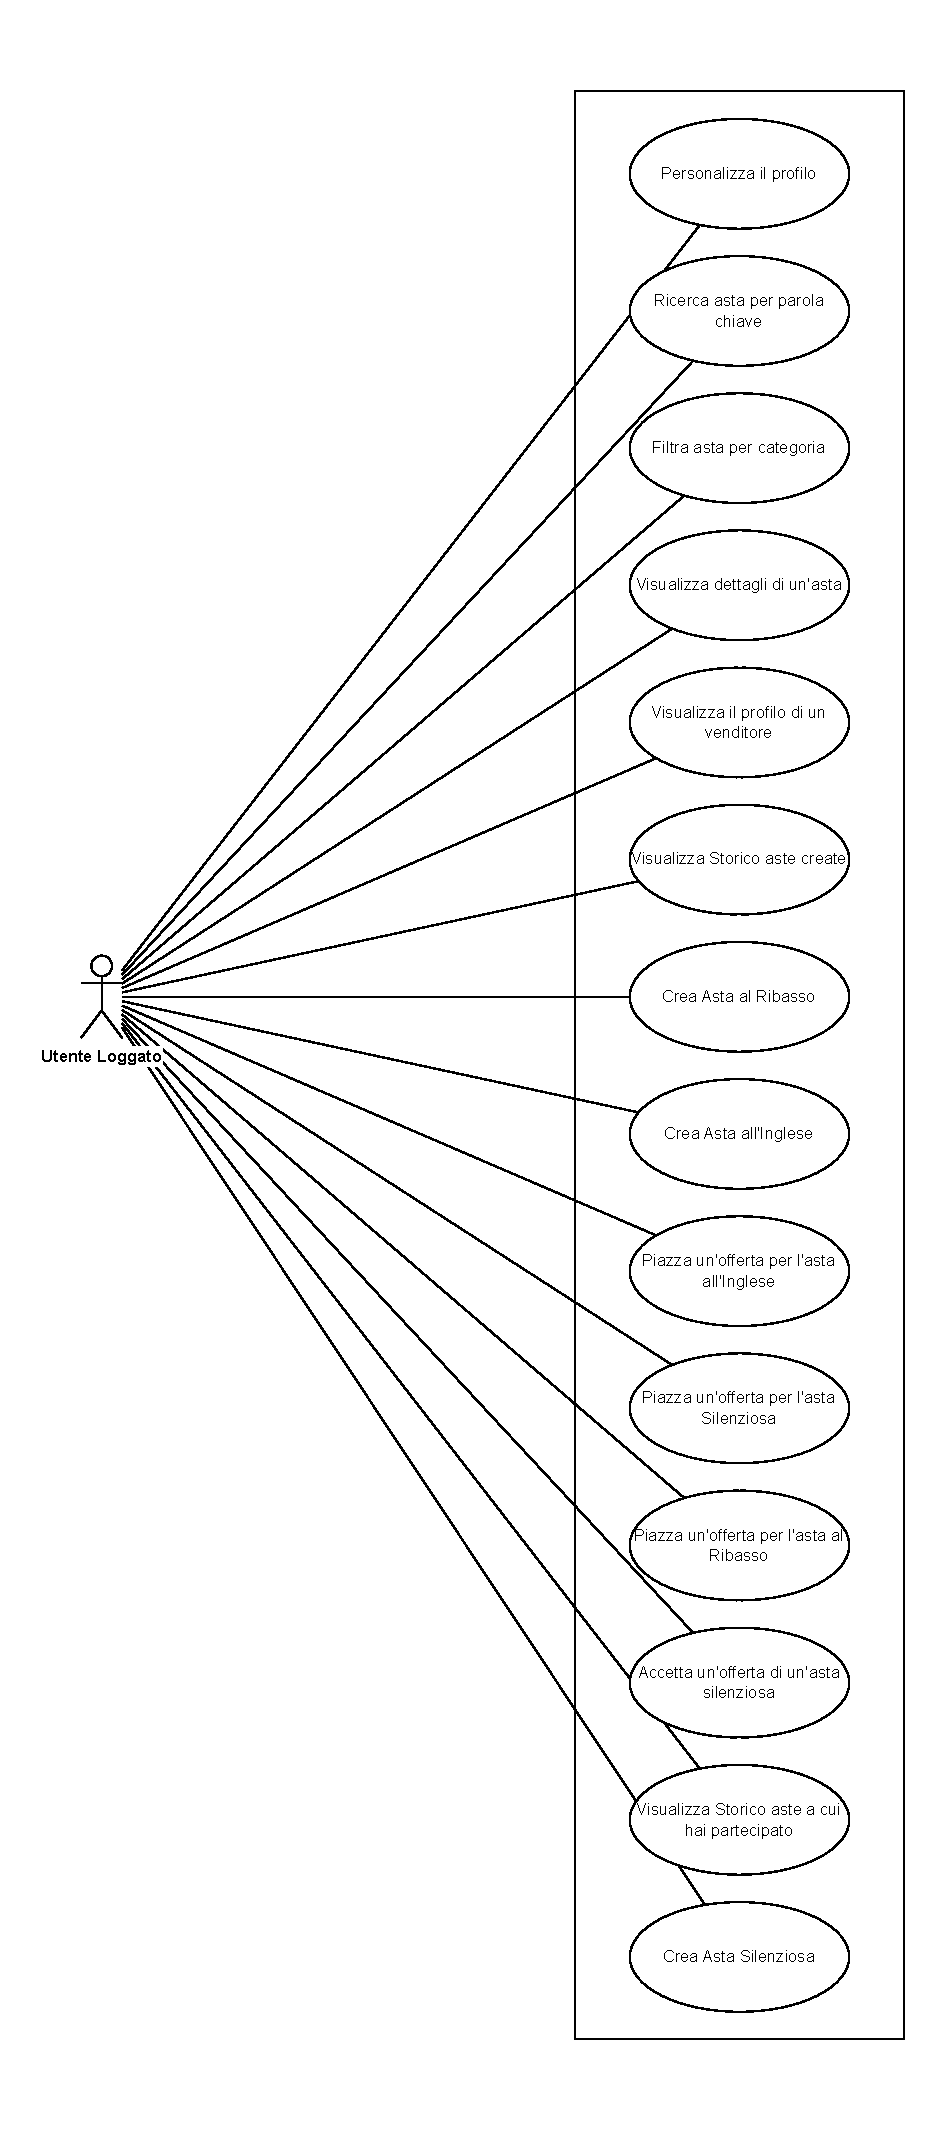
\includegraphics[width=.63\textwidth]{assets/utente_loggato_use_case.pdf}

\newpage

\section{Tabelle di Cockburn}
\subsection{Creazione asta silenziosa}
\begin{table}[H]
	\renewcommand{\arraystretch}{1.3}
	\begin{tabularx}{\linewidth}{|p{135pt}|p{25pt}|>{\raggedright\arraybackslash}X|>{\raggedright\arraybackslash}X|}
		\hline \rowcolor[HTML]{DCDCDC}
		\textbf{\large\sffamily Use Case {\ttfamily \#}01}                            & \multicolumn{3}{>{\raggedright\arraybackslash}p{\dimexpr 0.5\linewidth+95.8pt\relax}|}{\textbf{\large\sffamily Creazione asta silenziosa}}                                                                                                                                                                                                 \\
		\hline Goal in Context                                                        & \multicolumn{3}{>{\raggedright\arraybackslash}p{\dimexpr 0.5\linewidth+95.8pt\relax}|}{L'utente vuole creare un'asta silenziosa.}                                                                                                                                                                                                          \\
		\hline Preconditions                                                          & \multicolumn{3}{>{\raggedright\arraybackslash}p{\dimexpr 0.5\linewidth+95.8pt\relax}|}{L'utente deve aver effettuato l'accesso.}                                                                                                                                                                                                           \\
		\hline Success End Conditions                                                 & \multicolumn{3}{>{\raggedright\arraybackslash}p{\dimexpr 0.5\linewidth+95.8pt\relax}|}{L'utente crea correttamente l'asta silenziosa che poi sarà accessibile agli altri  utenti.}                                                                                                                                                         \\

		\hline \rowcolor[HTML]{DCDCDC}
		\multirow{1}{*}{}{\textbf{\sffamily Description}}                             & \textbf{\sffamily Step}                                                                                                                                                            & \textbf{\sffamily User Action}                                   & \textbf{\sffamily System}                                                          \\
		\cline{2-4}                                                                   & 1                                                                                                                                                                                  & Dal mockup "Homepage" preme il pulsante "Carica Asta".           &                                                                                    \\
		\cline{2-4}                                                                   & 2                                                                                                                                                                                  &                                                                  & Mostra il mockup "Carica Asta" con 3 possibili scelte.                             \\
		\cline{2-4}                                                                   & 3                                                                                                                                                                                  & Seleziona il pulsante "Crea Asta silenziosa"                     &                                                                                    \\
		\cline{2-4}                                                                   & 4                                                                                                                                                                                  &                                                                  & Mostra il mockup "Creazione Asta silenziosa"                                       \\
		\cline{2-4}                                                                   & 5                                                                                                                                                                                  & Inserisce tutti i dati necessari e preme il pulsante "Crea Asta" &                                                                                    \\
		\cline{2-4}                                                                   & 6                                                                                                                                                                                  &                                                                  & Mostra un popup con l'esito della creazione dell'asta e torna al mockup "Homepage" \\

		\hline \rowcolor[HTML]{DCDCDC}
		\textbf{\sffamily Extensions}                                                 & \textbf{\sffamily Step}                                                                                                                                                            & \textbf{\sffamily User Action}                                   & \textbf{\sffamily System}                                                          \\
		\hline
		\multirow{2}{135pt}{\raggedright\arraybackslash Dati mancanti o non corretti} & 5.a                                                                                                                                                                                &                                                                  & Mostra un popup di errore                                                          \\
		\cline{2-4}                                                                   & 5.b                                                                                                                                                                                & Visualizza il popup e riprova l'inserimento dei dati             &                                                                                    \\

		\hline
	\end{tabularx}
\end{table}

\newpage
\subsection{Offerta asta silenziosa}
\begin{table}[H]
	\renewcommand{\arraystretch}{1.3}
	\begin{tabularx}{\linewidth}{|p{135pt}|p{25pt}|>{\raggedright\arraybackslash}X|>{\raggedright\arraybackslash}X|}
		\hline \rowcolor[HTML]{DCDCDC}
		\textbf{\large\sffamily Use Case {\ttfamily \#}02}                               & \multicolumn{3}{>{\raggedright\arraybackslash}p{\dimexpr 0.5\linewidth+95.8pt\relax}|}{\textbf{\large\sffamily Offerta asta silenziosa}}                                                                                                                                                                                                                   \\
		\hline Goal in Context                                                           & \multicolumn{3}{>{\raggedright\arraybackslash}p{\dimexpr 0.5\linewidth+95.8pt\relax}|}{ L'utente vuole piazzare un'offerta per un'asta silenziosa }                                                                                                                                                                                                        \\
		\hline Preconditions                                                             & \multicolumn{3}{>{\raggedright\arraybackslash}p{\dimexpr 0.5\linewidth+95.8pt\relax}|}{ L'utente deve aver effettuato l'accesso e si deve trovare nella pagina "Home"}                                                                                                                                                                                     \\
		\hline Success End Conditions                                                    & \multicolumn{3}{>{\raggedright\arraybackslash}p{\dimexpr 0.5\linewidth+95.8pt\relax}|}{ L'utente piazzà correttamente l'offerta che sarà visibile al venditore }                                                                                                                                                                                           \\

		\hline \rowcolor[HTML]{DCDCDC}
		\multirow{1}{*}{}{\textbf{\sffamily Description}}                                & \textbf{\sffamily Step}                                                                                                                                                & \textbf{\sffamily User Action}                                                   & \textbf{\sffamily System}                                                                      \\
		\cline{2-4}                                                                      & 1                                                                                                                                                                      & Preme sull'asta su cui vuole fare un'offerta.                                    &                                                                                                \\
		\cline{2-4}                                                                      & 2                                                                                                                                                                      &                                                                                  & Mostra il mockup "Dettaglio asta silenziosa" dove visualizzerà i dettagli dell'asta            \\
		\cline{2-4}                                                                      & 3                                                                                                                                                                      & Inserisce l'importo che vuole puntare e poi preme il pulsante "Conferma offerta" &                                                                                                \\
		\cline{2-4}                                                                      & 4                                                                                                                                                                      &                                                                                  & Il sistema mostra un messaggio di successo (mockup "Dettaglio asta silenziosa - success")      \\
		\cline{2-4}                                                                      & 5                                                                                                                                                                      & Preme il pulsante "ok"                                                           &                                                                                                \\
		\cline{2-4}                                                                      & 6                                                                                                                                                                      &                                                                                  & Il sistema riporta l'utente alla pagina home                                                   \\

		\hline \rowcolor[HTML]{DCDCDC}
		\textbf{\sffamily Extensions}                                                    & \textbf{\sffamily Step}                                                                                                                                                & \textbf{\sffamily User Action}                                                   & \textbf{\sffamily System}                                                                      \\
		\hline
		\multirow{3}{135pt}{La puntata non va a buon fine, qualsiasi sia stato l'errore} & 3.a                                                                                                                                                                    &                                                                                  & Il sistema mostra una finestra indicando l'errore (mockup "Dettaglio asta silenziosa - error") \\
		\cline{2-4}                                                                      & 3.b                                                                                                                                                                    & Preme il pulsante "ok"                                                           &                                                                                                \\
		\cline{2-4}                                                                      & 3.c                                                                                                                                                                    &                                                                                  & Il sistema chiude questa finestra senza cambiare pagina.                                       \\

		\hline
	\end{tabularx}
\end{table}

\newpage
\subsection{Aggiungere link social}
\begin{table}[H]
	\renewcommand{\arraystretch}{1.3}
	\begin{tabularx}{\linewidth}{|p{135pt}|p{25pt}|>{\raggedright\arraybackslash}X|>{\raggedright\arraybackslash}X|}
		\hline \rowcolor[HTML]{DCDCDC}
		\textbf{\large\sffamily Use Case {\ttfamily \#}03} & \multicolumn{3}{>{\raggedright\arraybackslash}p{\dimexpr 0.5\linewidth+95.8pt\relax}|}{\textbf{\large\sffamily Aggiungere link social}}                                                                                                                                                                                   \\
		\hline Goal in Context                             & \multicolumn{3}{>{\raggedright\arraybackslash}p{\dimexpr 0.5\linewidth+95.8pt\relax}|}{ L'utente vuole aggiungere un nuovo link social }                                                                                                                                                                                  \\
		\hline Preconditions                               & \multicolumn{3}{>{\raggedright\arraybackslash}p{\dimexpr 0.5\linewidth+95.8pt\relax}|}{ L'utente deve aver effettuato l'accesso e si deve trovare nella pagina "Profilo" }                                                                                                                                                \\
		\hline Success End Conditions                      & \multicolumn{3}{>{\raggedright\arraybackslash}p{\dimexpr 0.5\linewidth+95.8pt\relax}|}{ L'utente inserisce correttamente un nuovo link social }                                                                                                                                                                           \\

		\hline \rowcolor[HTML]{DCDCDC}
		\multirow{1}{*}{}{\textbf{\sffamily Description}}  & \textbf{\sffamily Step}                                                                                                                                                    & \textbf{\sffamily User Action}                   & \textbf{\sffamily System}                                                                 \\
		\cline{2-4}                                        & 1                                                                                                                                                                          & Preme il pulsante "Modifica"                     &                                                                                           \\
		\cline{2-4}                                        & 2                                                                                                                                                                          &                                                  & Mostra il mockup "Profile Page - Modifica"                                                \\
		\cline{2-4}                                        & 3                                                                                                                                                                          & Preme il pulsante "aggiungi link"                &                                                                                           \\
		\cline{2-4}                                        & 4                                                                                                                                                                          &                                                  & Mostra il mockup "Profile Page - modifica - aggiungi link"                                \\
		\cline{2-4}                                        & 5                                                                                                                                                                          & Inserisce il link e preme il pulsante "Conferma" &                                                                                           \\
		\cline{2-4}                                        & 6                                                                                                                                                                          &                                                  & Ritorna al mockup precedente                                                              \\
		\cline{2-4}                                        & 7                                                                                                                                                                          & Preme il pulsante "salva"                        &                                                                                           \\
		\cline{2-4}                                        & 8                                                                                                                                                                          &                                                  & Torna alla pagina profilo                                                                 \\

		\hline \rowcolor[HTML]{DCDCDC}
		\textbf{\sffamily Extensions}                      & \textbf{\sffamily Step}                                                                                                                                                    & \textbf{\sffamily User Action}                   & \textbf{\sffamily System}                                                                 \\
		\hline
		\multirow{1}{135pt}{Link non valido}               & 5.a                                                                                                                                                                        &                                                  & Mostra il messaggio "Link non valido" appena sotto il campo di testo colorandolo di rosso \\
		\cline{2-4}                                        & 5.b                                                                                                                                                                        & Ripete lo step 5                                 &                                                                                           \\

		\hline
	\end{tabularx}
\end{table}

\newpage
\subsection{Visualizzazione delle aste create ancora attive}
\begin{table}[H]
	\renewcommand{\arraystretch}{1.3}
	\begin{tabularx}{\linewidth}{|p{135pt}|p{25pt}|>{\raggedright\arraybackslash}X|>{\raggedright\arraybackslash}X|}
		\hline \rowcolor[HTML]{DCDCDC}
		\textbf{\large\sffamily Use Case {\ttfamily \#}04}            & \multicolumn{3}{>{\raggedright\arraybackslash}p{\dimexpr 0.5\linewidth+95.8pt\relax}|}{\textbf{\large\sffamily Visualizzazione delle aste create ancora attive}}                                                                                                                                                                                                          \\
		\hline Goal in Context                                        & \multicolumn{3}{>{\raggedright\arraybackslash}p{\dimexpr 0.5\linewidth+95.8pt\relax}|}{ L'utente vuole visualizzare le aste da lui create che sono ancora in corso }                                                                                                                                                                                                      \\
		\hline Preconditions                                          & \multicolumn{3}{>{\raggedright\arraybackslash}p{\dimexpr 0.5\linewidth+95.8pt\relax}|}{ L'utente deve aver effettuato l'accesso}                                                                                                                                                                                                                                          \\
		\hline Success End Conditions                                 & \multicolumn{3}{>{\raggedright\arraybackslash}p{\dimexpr 0.5\linewidth+95.8pt\relax}|}{ L'utente visualizza correttamente le aste da lui create }                                                                                                                                                                                                                         \\

		\hline \rowcolor[HTML]{DCDCDC}
		\multirow{1}{*}{}{\textbf{\sffamily Description}}             & \textbf{\sffamily Step}                                                                                                                                              & \textbf{\sffamily User Action}                                                                                                           & \textbf{\sffamily System}                               \\
		\cline{2-4}                                                   & 1                                                                                                                                                                    & Preme sul pulsante "storico aste" nella barra di navigazione in basso                                                                    &                                                         \\
		\cline{2-4}                                                   & 2                                                                                                                                                                    &                                                                                                                                          & Mostra il mockup "Storico aste - acquistate"            \\
		\cline{2-4}                                                   & 3                                                                                                                                                                    & Preme il pulsante "Aste create"                                                                                                          &                                                         \\
		\cline{2-4}                                                   & 4                                                                                                                                                                    &                                                                                                                                          & Mostra il mockup "Storico aste - create"                \\
		\cline{2-4}                                                   & 5                                                                                                                                                                    & L'utente visualizza le aste che ha creato e riconosce quelle attive grazie a un riquadro blu in alto a destra con la dicitura "in corso" &                                                         \\

		\hline \rowcolor[HTML]{DCDCDC}
		\textbf{\sffamily Extensions}                                 & \textbf{\sffamily Step}                                                                                                                                              & \textbf{\sffamily User Action}                                                                                                           & \textbf{\sffamily System}                               \\
		\hline\multirow{2}{135pt}{L'utente non ha ancora creato aste} & 4.a                                                                                                                                                                  &                                                                                                                                          & Mostra il messaggio "Non hai ancora creato nessun'asta" \\

		\hline
	\end{tabularx}
\end{table}

\newpage

\section{Mockup del Software}
I mock-up sono stati progettati con Figma. Di seguito viene riportata la lista completa dei prototipi realizzati.

\subsection{Accesso e registrazione}
Il primo mockup mostra la schermata di accesso dov'è possibile accedere con email e password oppure tramite google.
Inoltre, è presente un pulsante per navigare alla pagina di registrazione.\sskip
Il secondo mockup mostra la schermata di registrazione dove l'utente compilerà i vari campi e premere il pulsante "Registrati" per confermare la registrazione.
Inoltre, è presente un pulsante per navigare alla pagina di accesso.
\begin{center}
	\begin{tabular}{cc}
		Accesso                                                          &
		Registrazione                                                          \\
		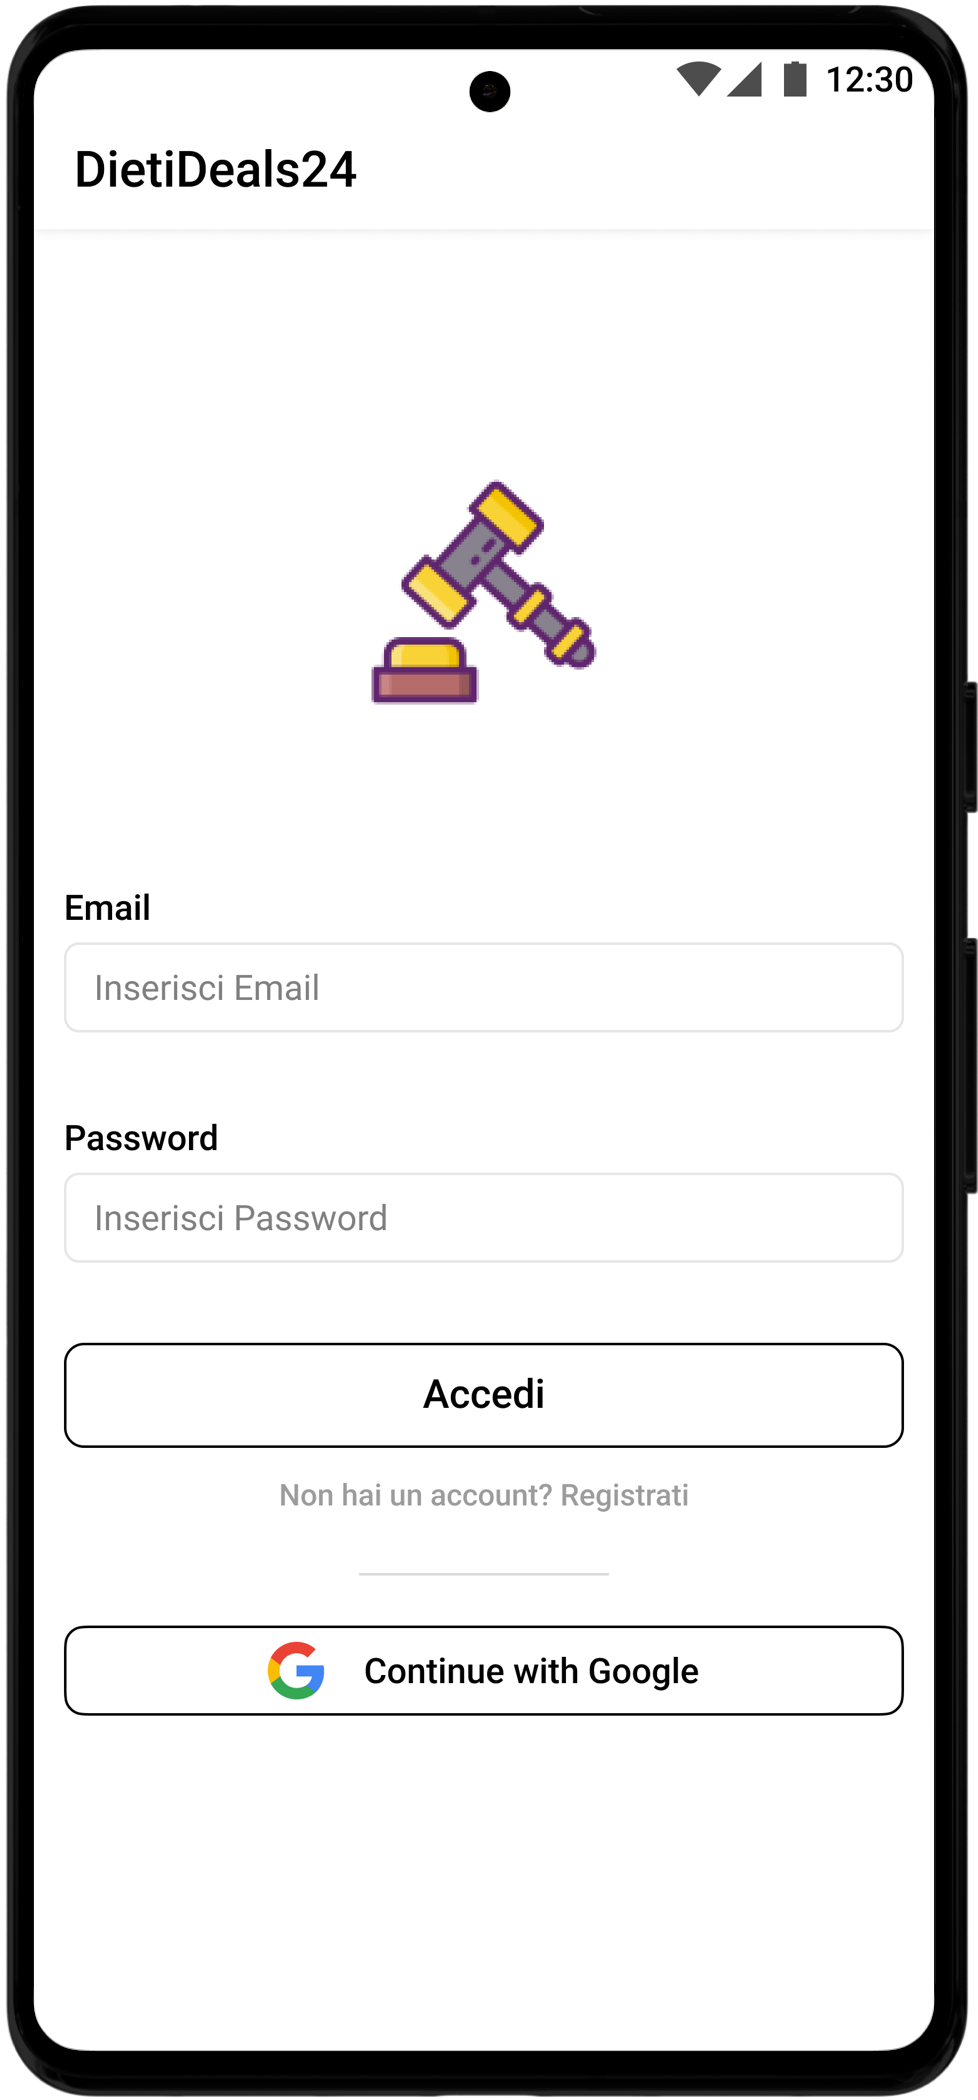
\includegraphics[width=.35\textwidth]{assets/mockup/Accesso.png} &
		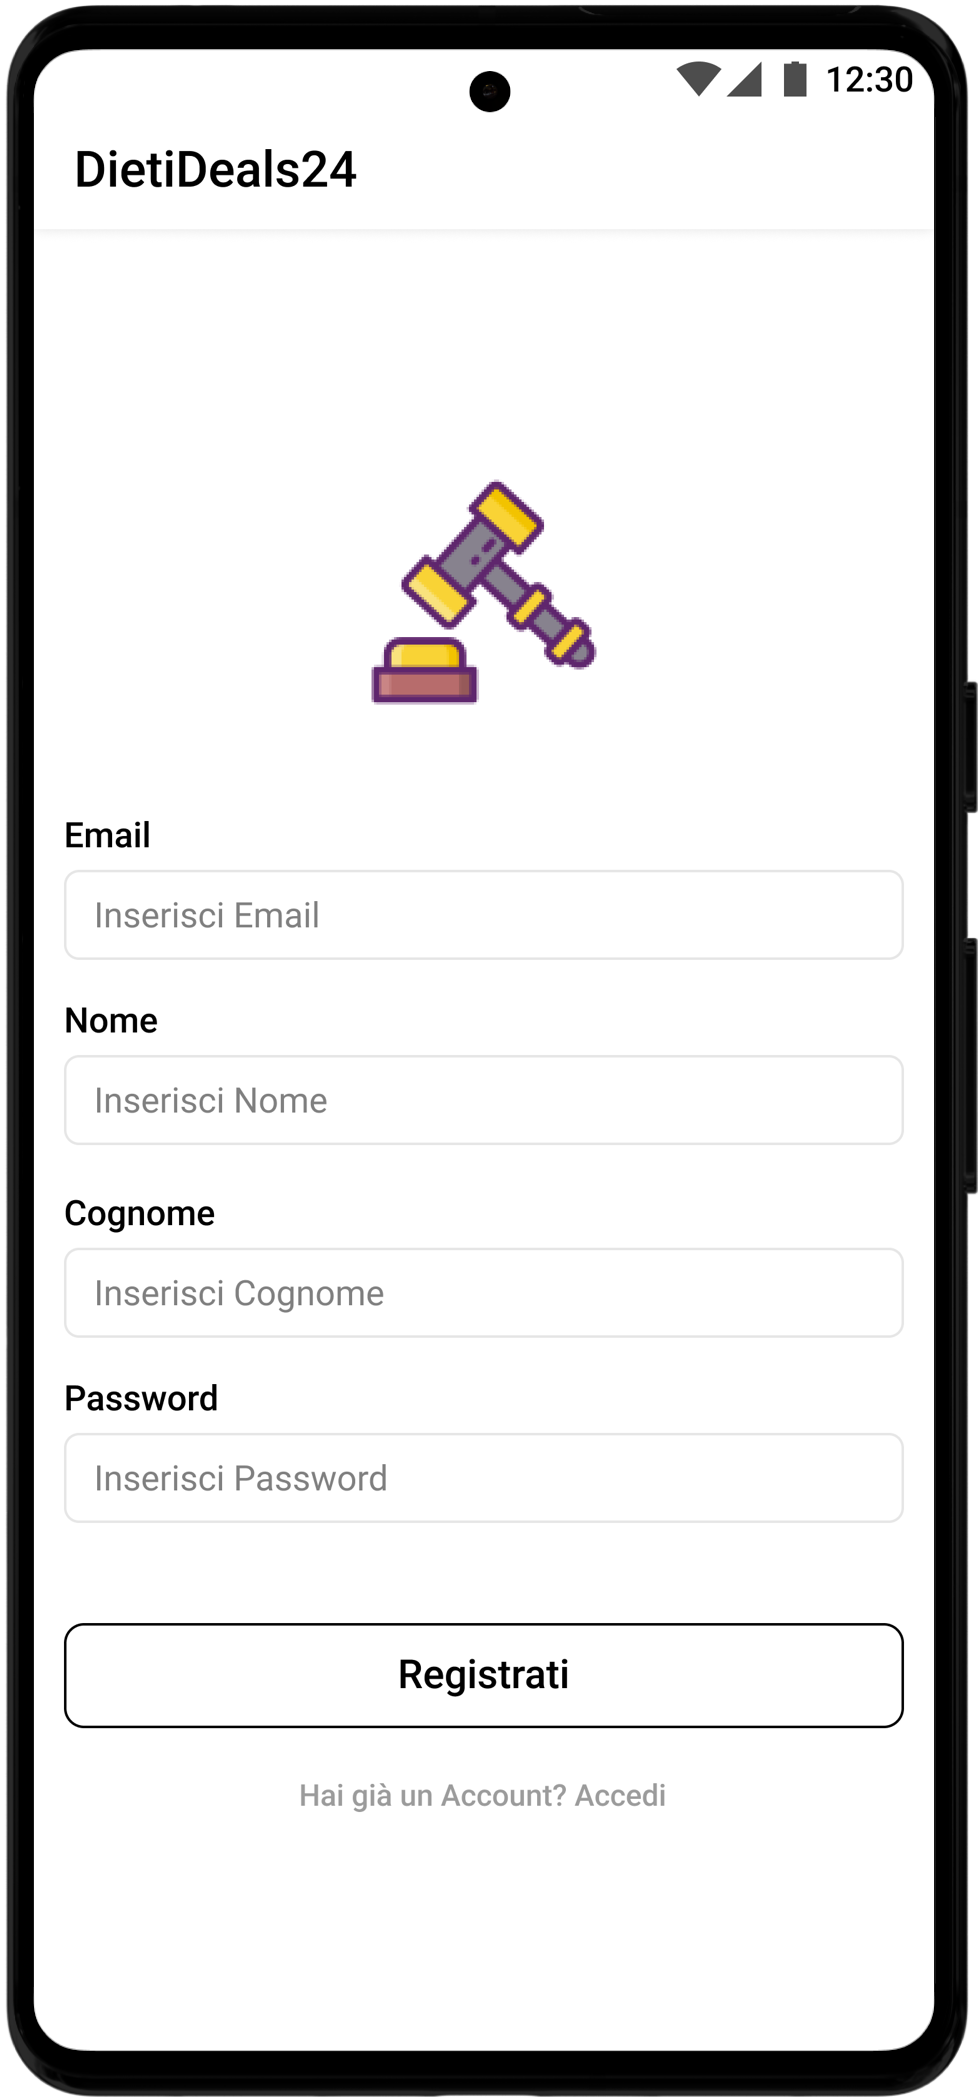
\includegraphics[width=.35\textwidth]{assets/mockup/Registrazione.png} \\
	\end{tabular}
\end{center}

\newpage
\subsection{Home}
Il mockup mostra la pagina principale dell'app, progettata per visualizzare e interagire con le aste in corso.
Questi sono gli elementi chiave:
\begin{itemize}
	\item Una barra di ricerca in alto per cercare le aste in base alla loro descrizioni.
	\item La lista delle categorie scorrevele orizzontalmente, cliccando su una di queste, verranno mostrate solo le aste di quella categoria.
	\item Una sezione "Aste in Corso" che mostra le aste attive.
\end{itemize}
\begin{center}
	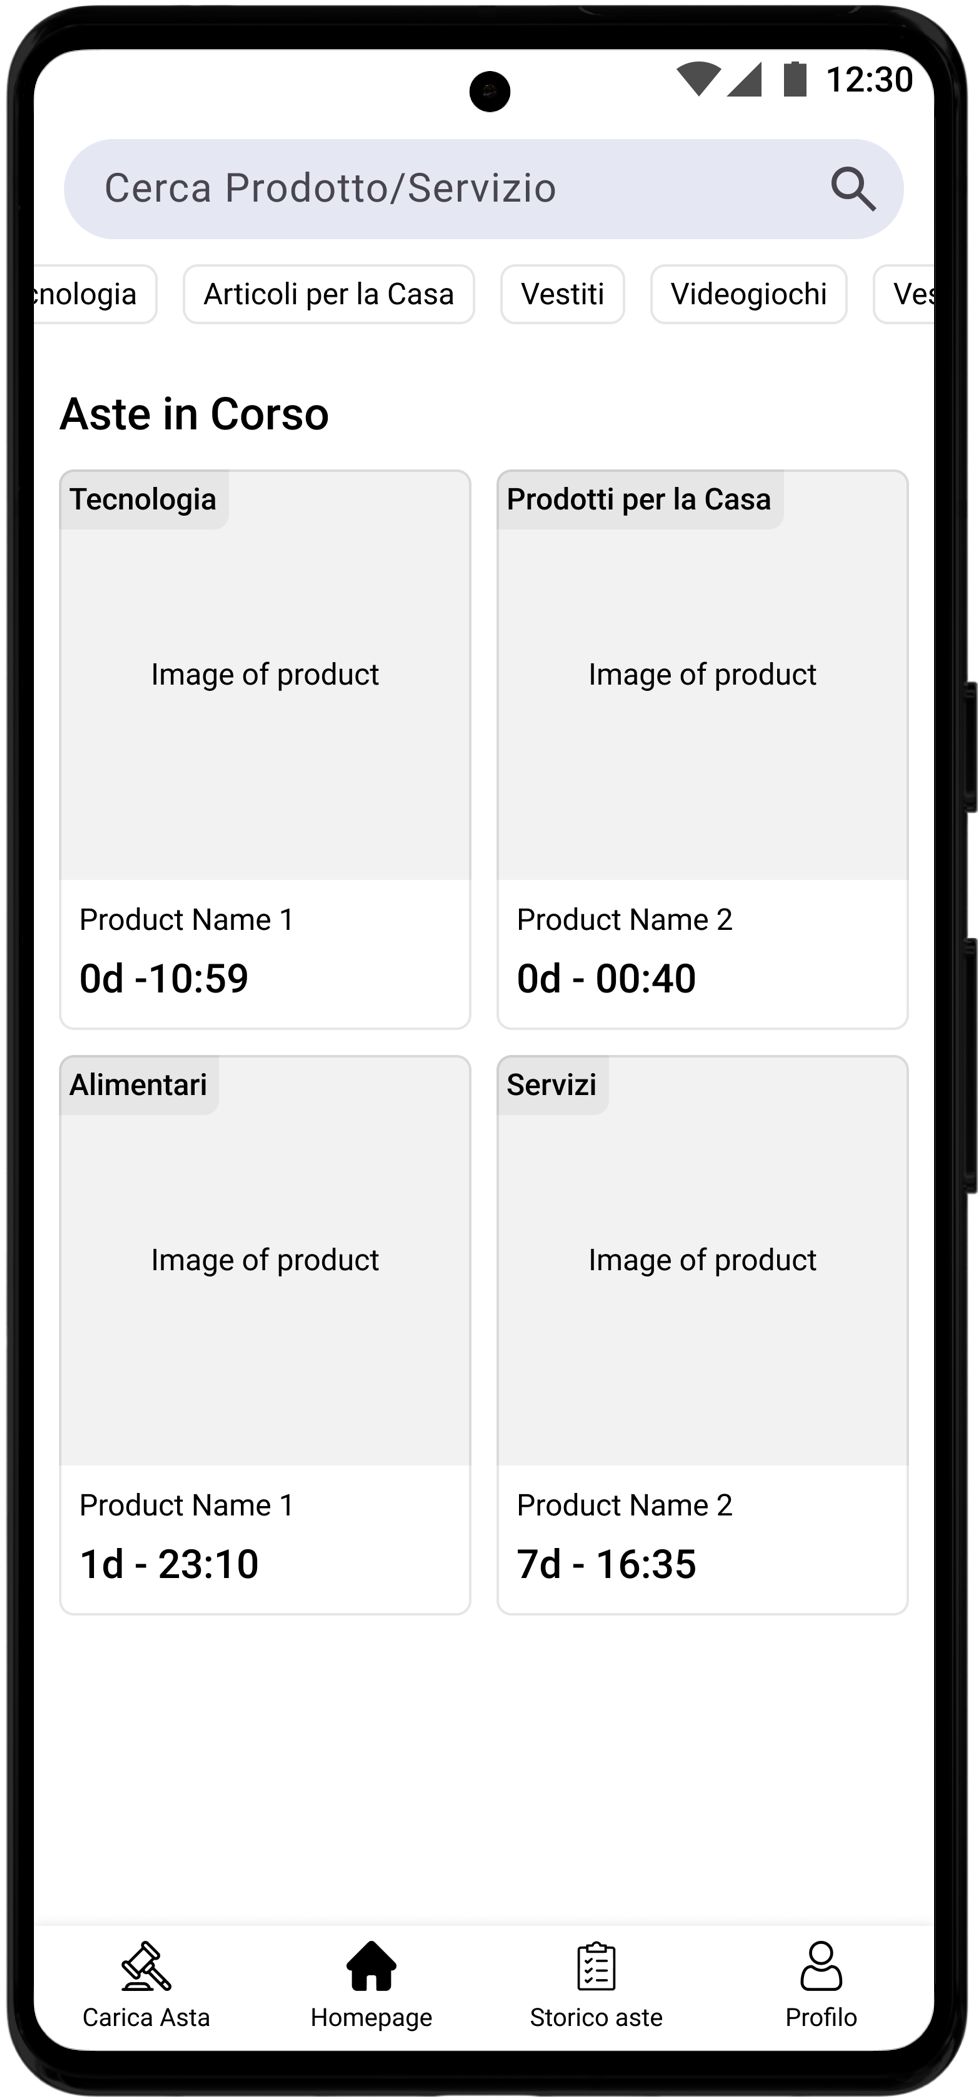
\includegraphics[width=.35\textwidth]{assets/mockup/HomePage.png}
\end{center}

\newpage
\subsection{Storico aste}
L'interfaccia è progettata per essere intuitiva e facilmente navigabile, permettendo agli utenti di visualizzare rapidamente le informazioni essenziali sulle loro aste, sia quelle a cui hanno partecipato come acquirenti, sia quelle che hanno creato come venditori.\\
È possibile scorrere tra la lista delle aste acquistate e quelle create, mediante la barra di navigazione posta in alto oppure scorrendo verso destra o sinistra.

\begin{center}
	\begin{tabular}{cc}
		Aste acquistate                                                                    &
		Aste create                                                                          \\
		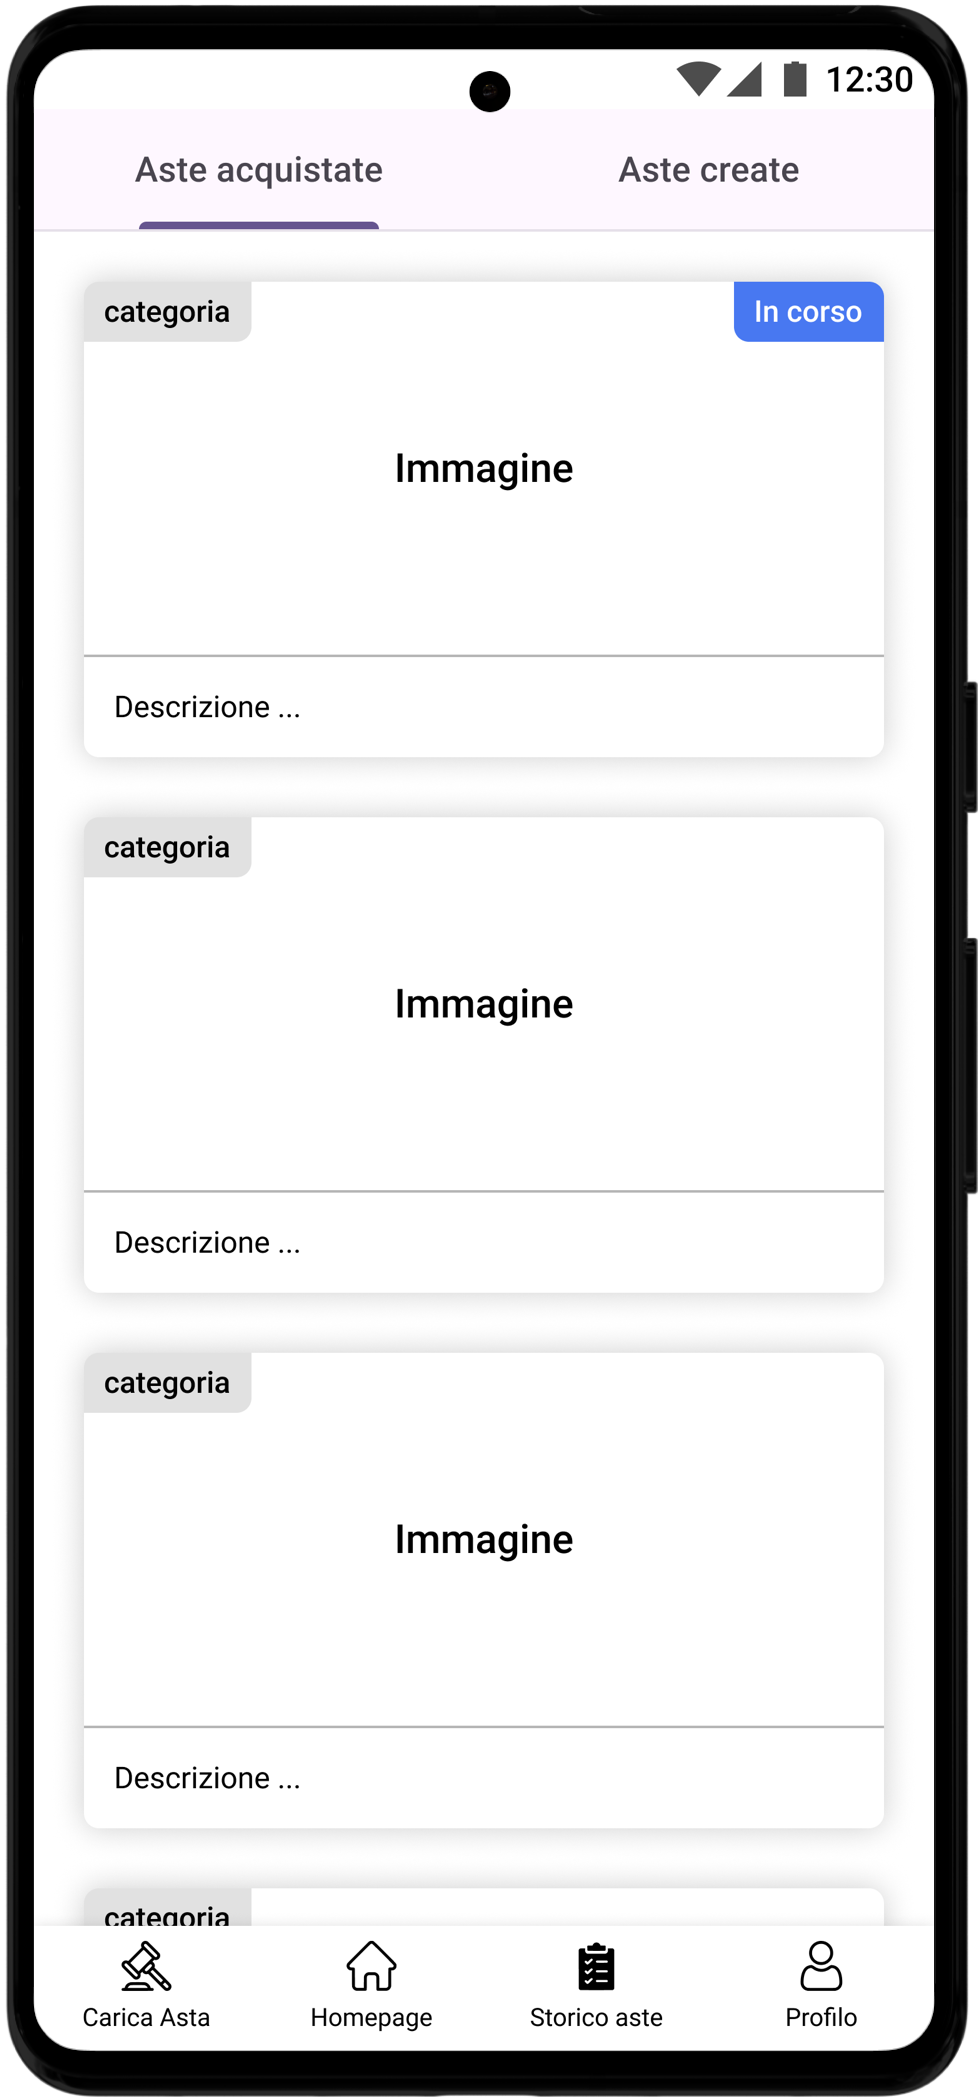
\includegraphics[width=.35\textwidth]{assets/mockup/Storico aste - acquistate.png} &
		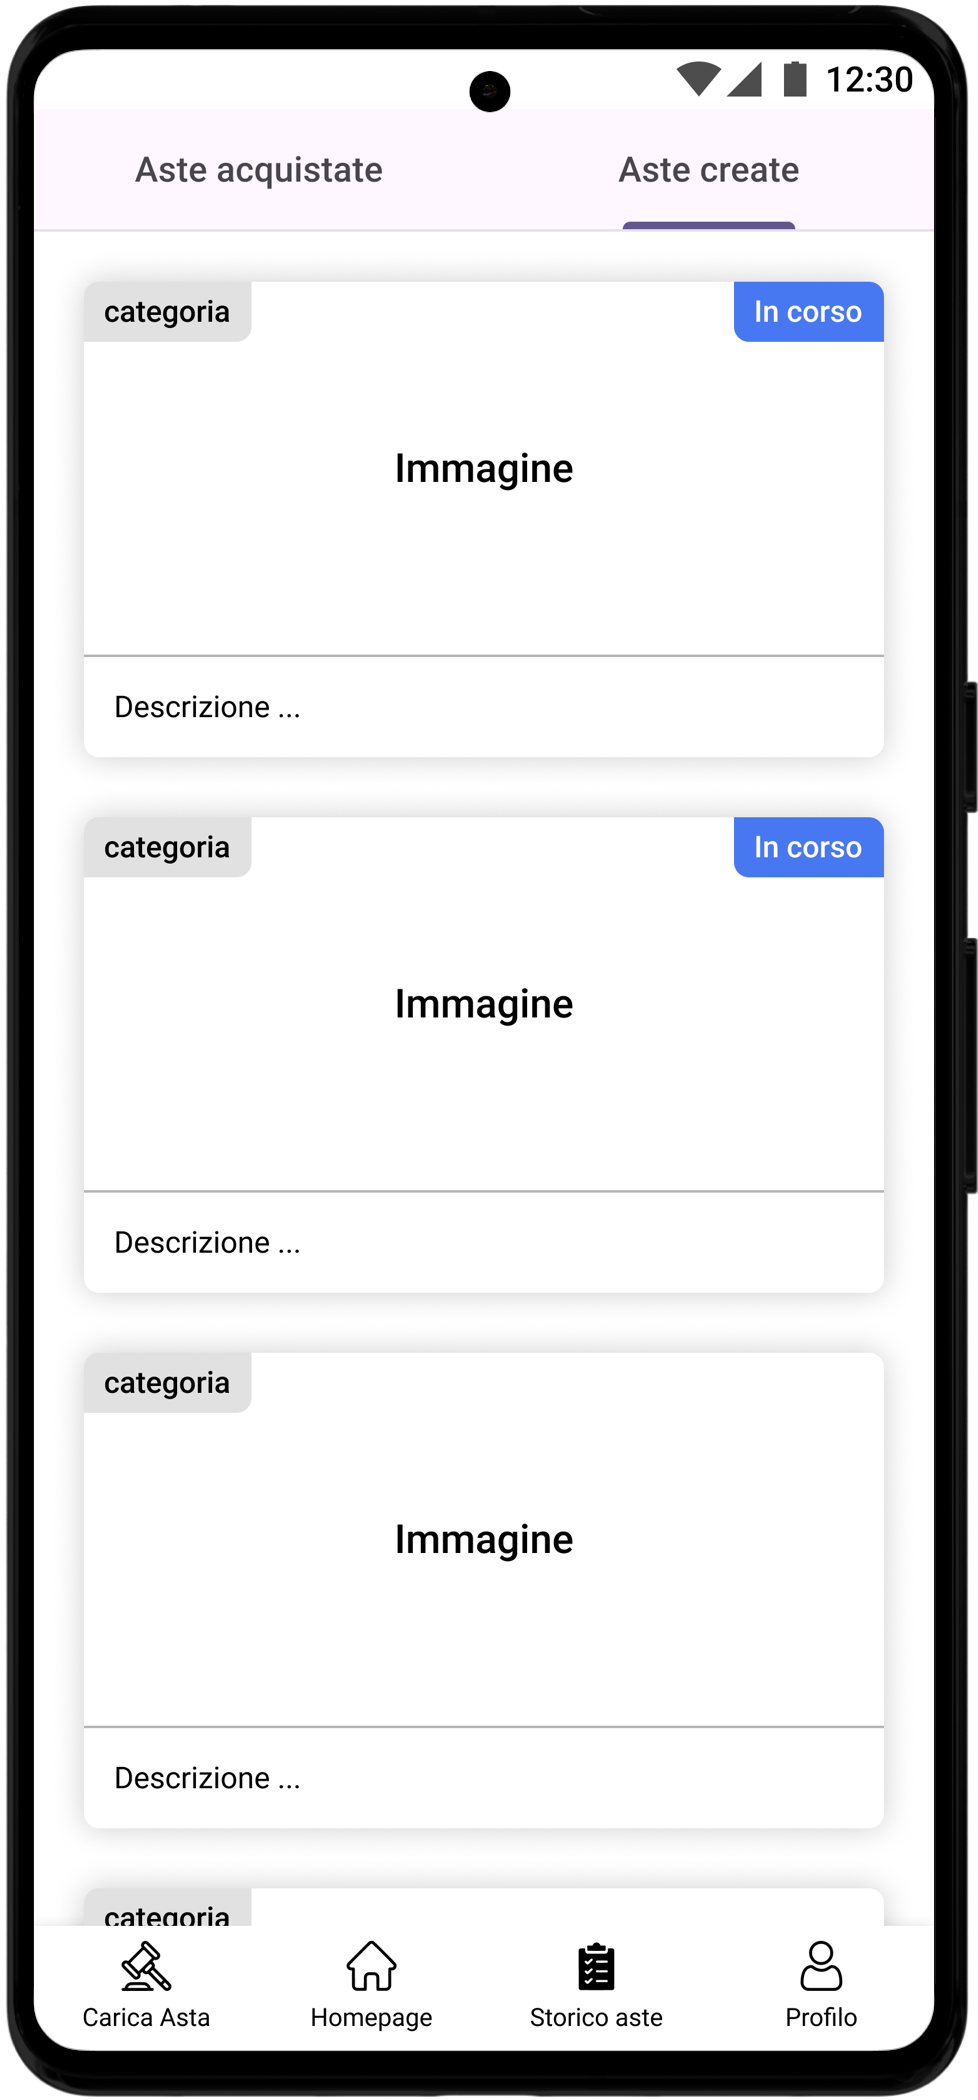
\includegraphics[width=.35\textwidth]{assets/mockup/Storico aste - create.png}       \\
	\end{tabular}
\end{center}

\newpage
\subsection{Profilo}
Il mockup "Profilo" mostra le informazioni personali dell'utente loggato.\\
Premendo il pulsante "Modifica" verrà mostrato il mockup "Modifica profilo" dove l'utente può modificare nome, cognome, bio, link al proprio sito e link ai profili social.
Premendo su "Aggiungi link" verrà mostrato il terzo mockup dove inserirà un nuovo link social.\meskip
Infine premerà il tasto "Salva" per salvare le modifica effettuate.

\begin{center}
	\begin{tabular}{ccc}
		Profilo                                                                         &
		Modifica Profilo                                                                &
		Aggiungi link                                                                                   \\
		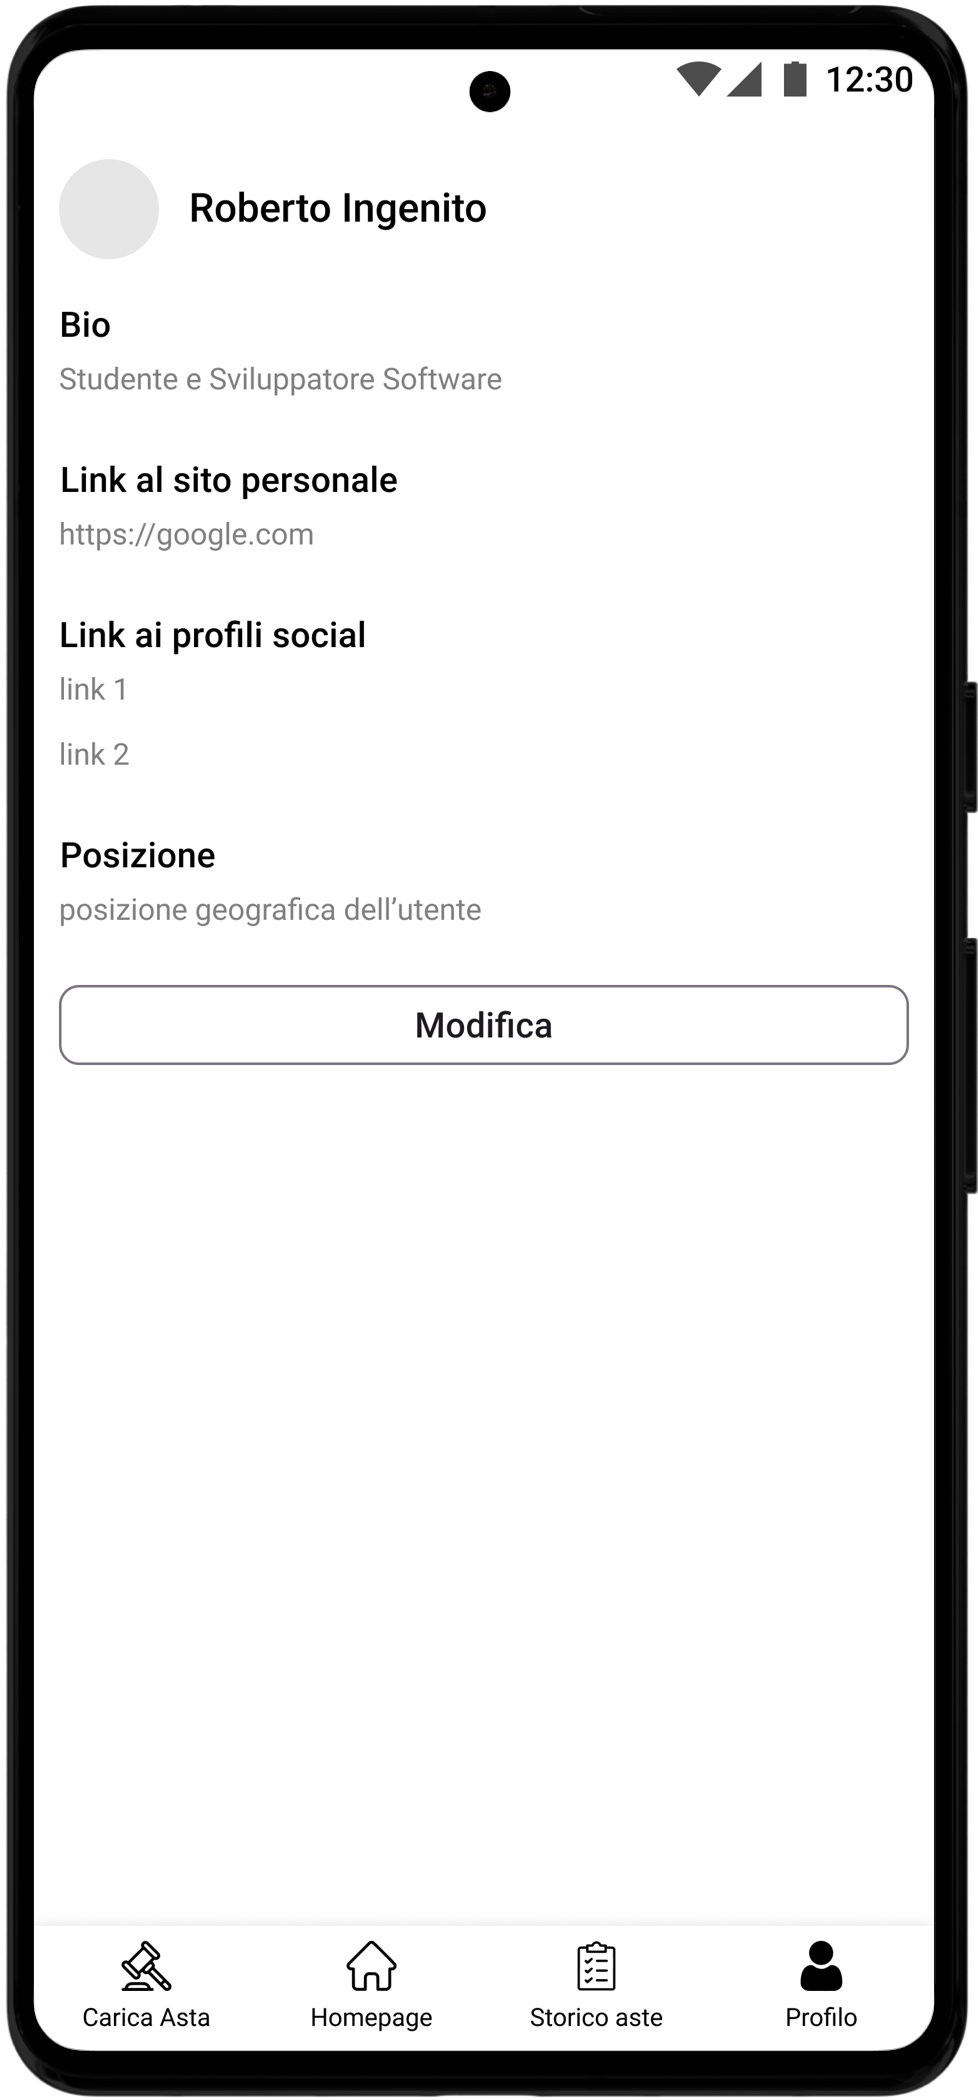
\includegraphics[width=.3\textwidth]{assets/mockup/Profile Page.png}            &
		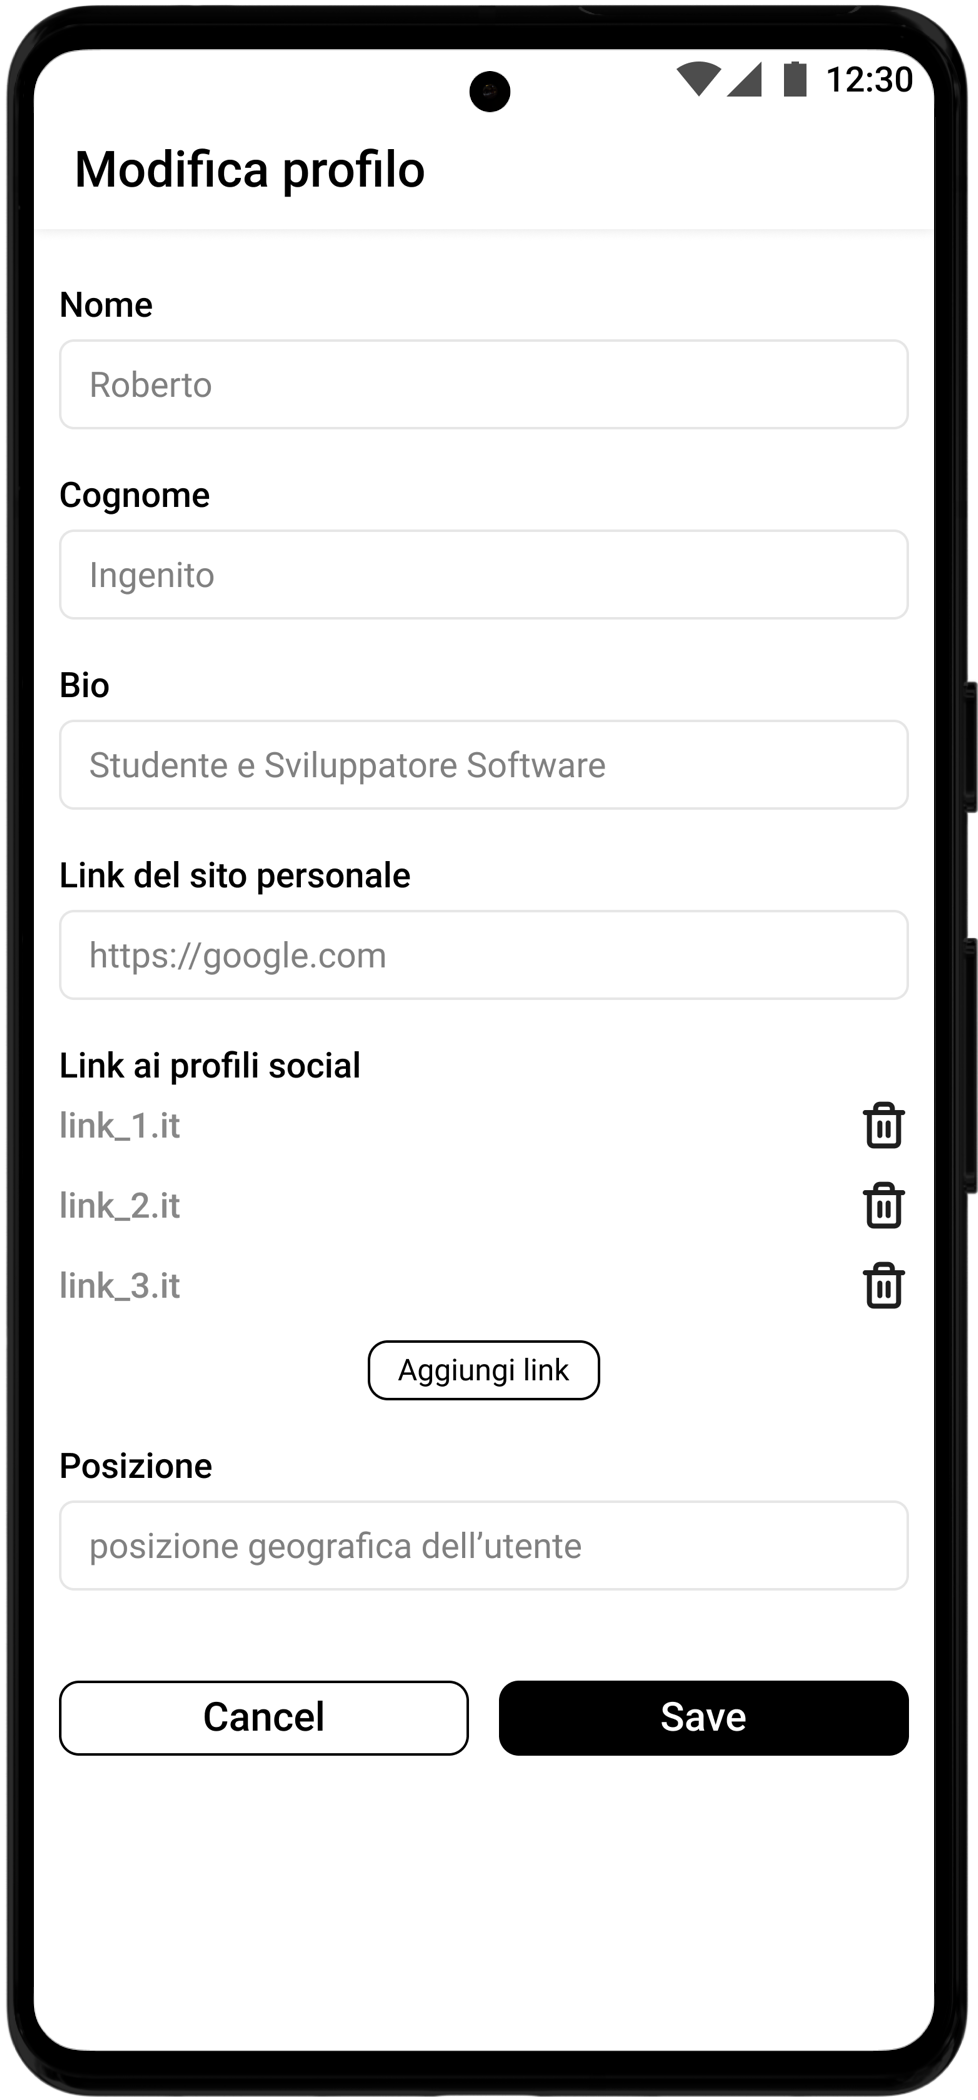
\includegraphics[width=.3\textwidth]{assets/mockup/Profile Page - modifica.png} &
		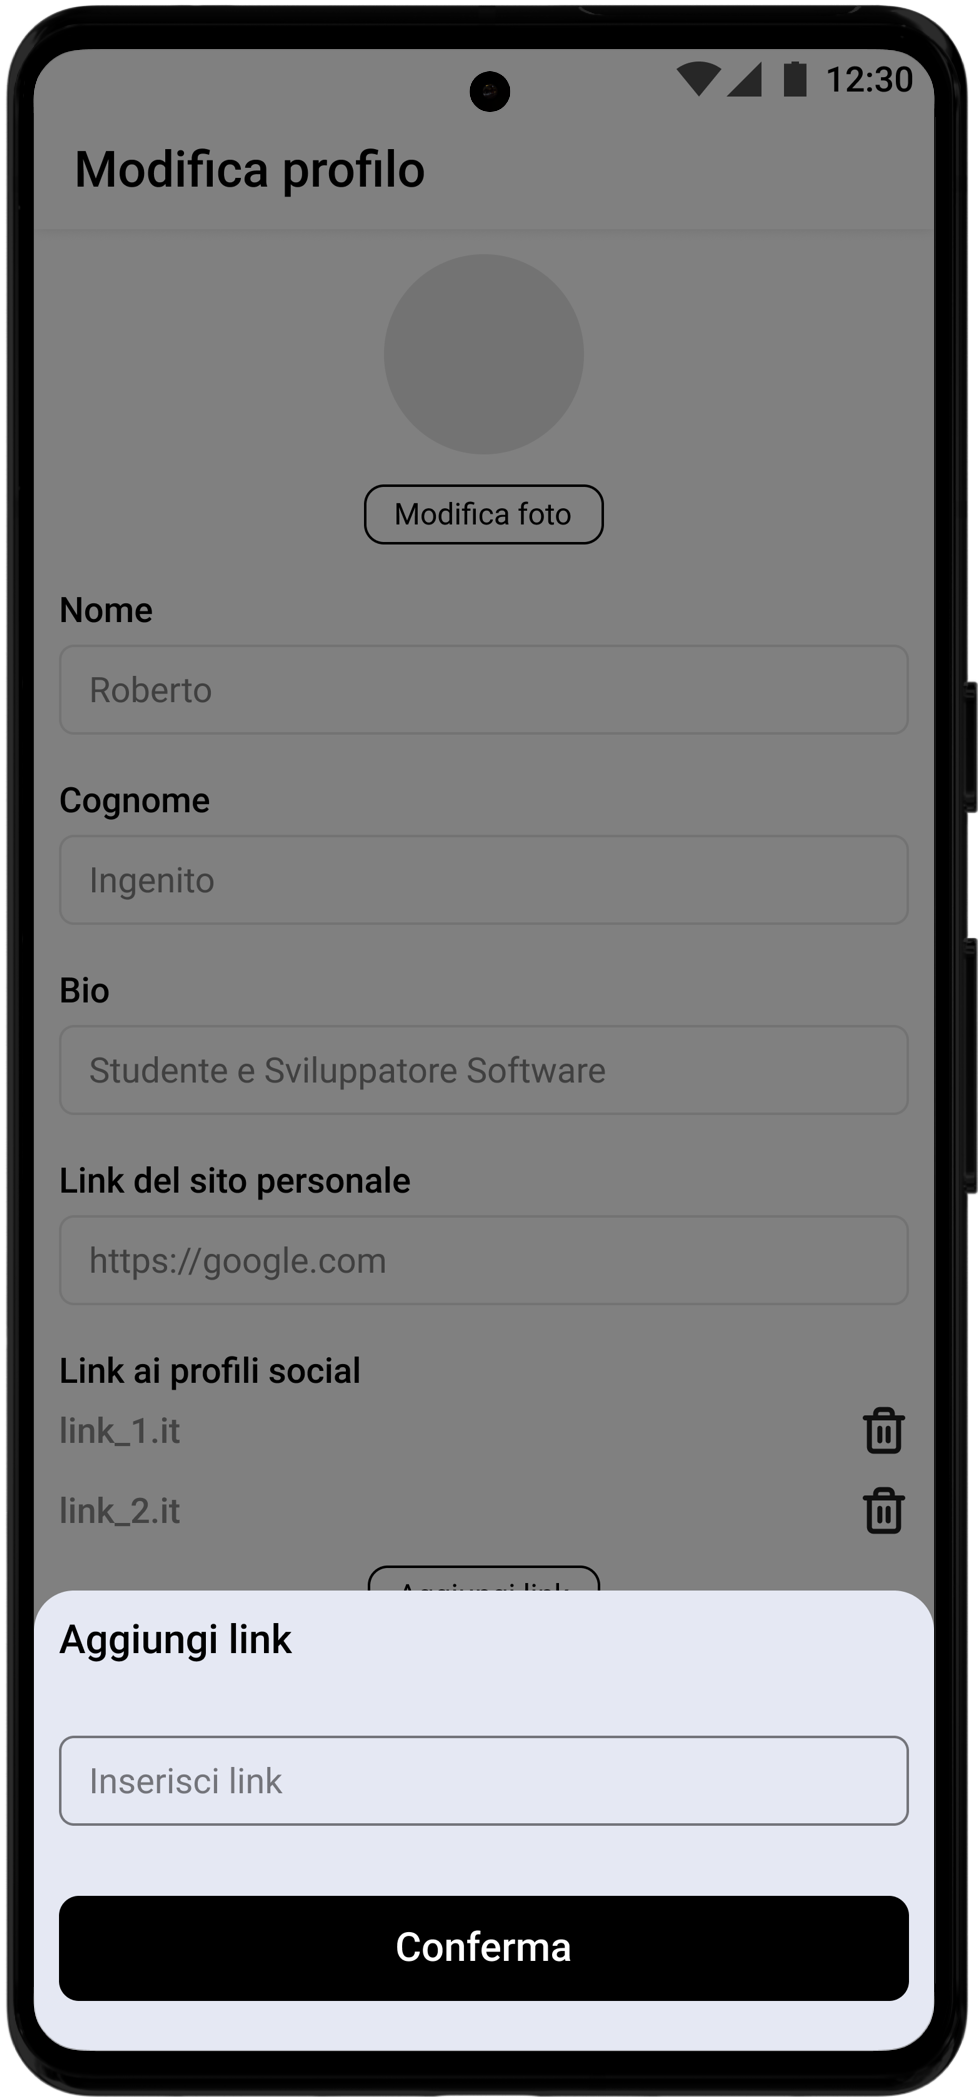
\includegraphics[width=.3\textwidth]{assets/mockup/Profile Page - modifica - aggiungi link.png} \\
	\end{tabular}
\end{center}

\newpage
\subsection{Piazzare un'offerta}
Dalla pagina Home, premendo su un'asta, l'applicazione navigherà a una di queste tre pagine a seconda del tipo di asta.\\
In base al tipo di asta, l'utente inserira l'importo della sua offerta oppure l'acquisterà direttamente (nel caso dell'asta al ribasso)

\begin{center}
	\begin{tabular}{ccc}
		Asta all'Inglese                                                                   &
		Asta al Ribasso                                                                    &
		Asta Silenziosa                                                                      \\
		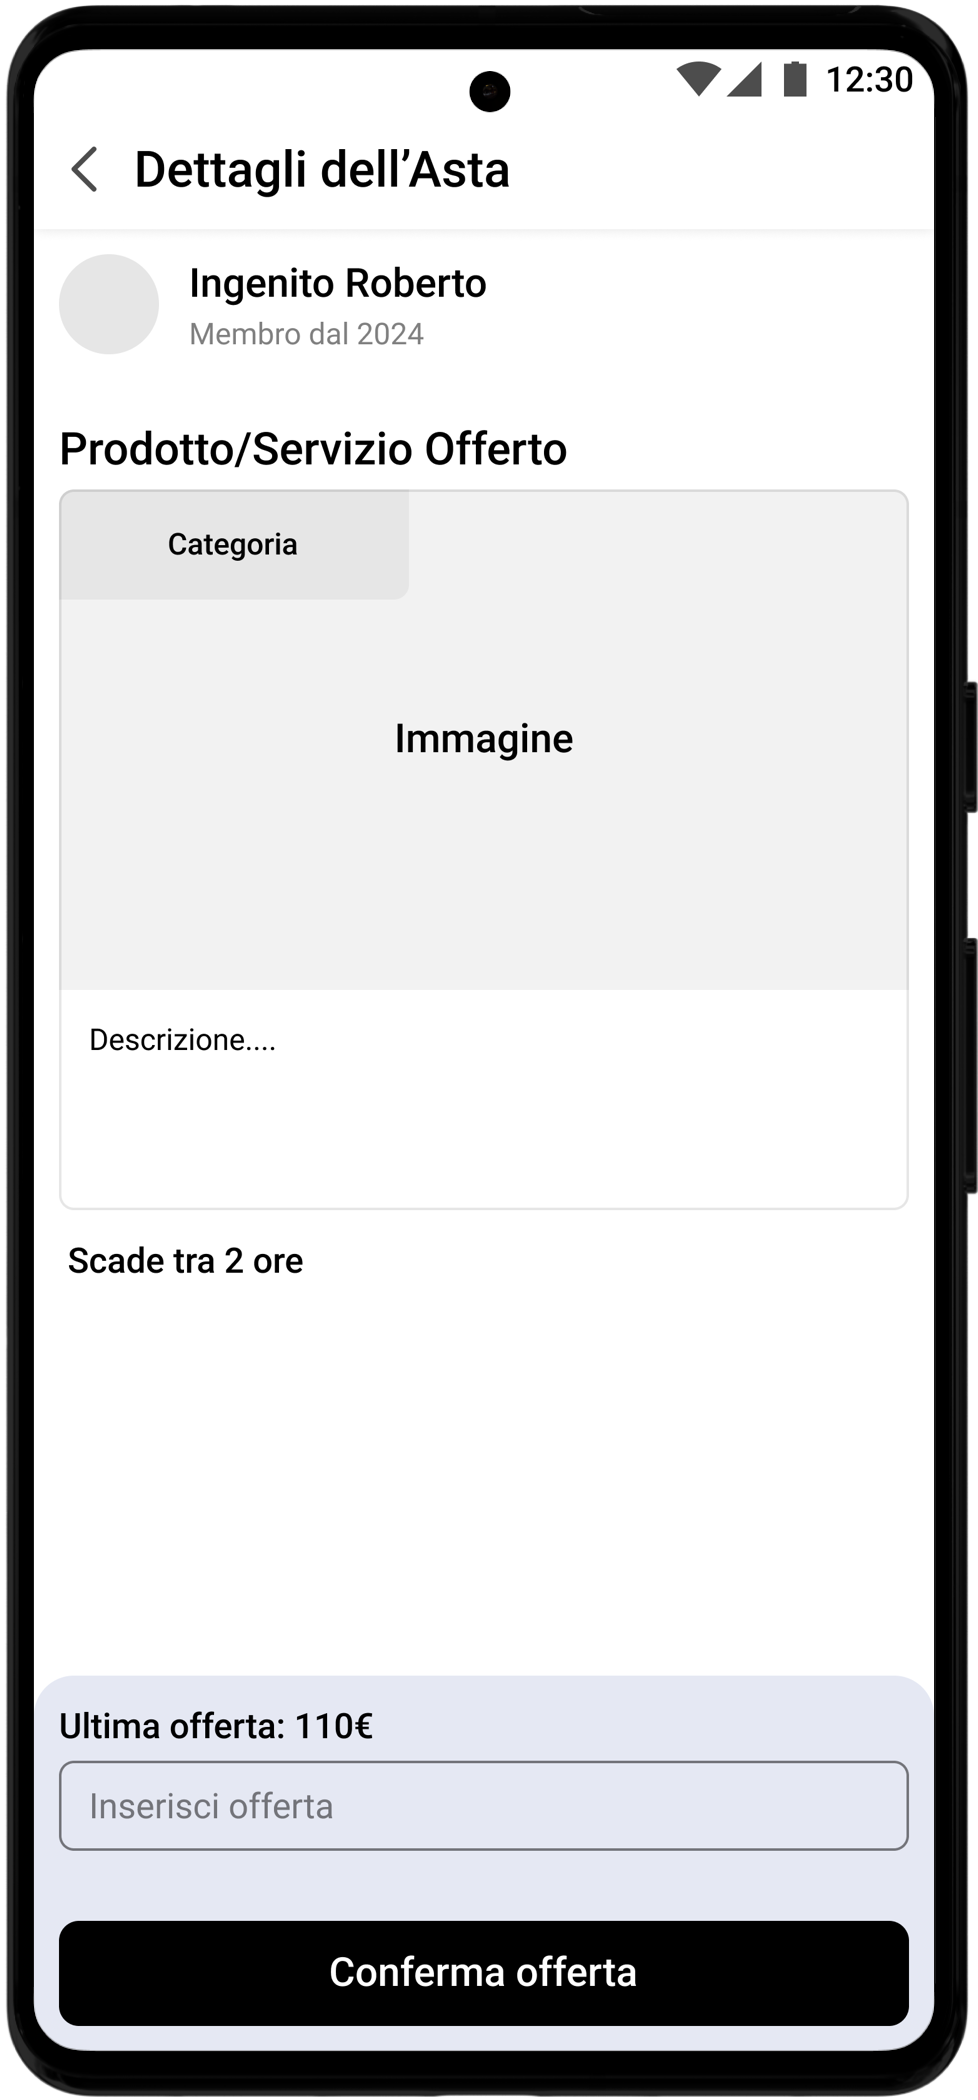
\includegraphics[width=.3\textwidth]{assets/mockup/Dettaglio Asta all'Inglese.png} &
		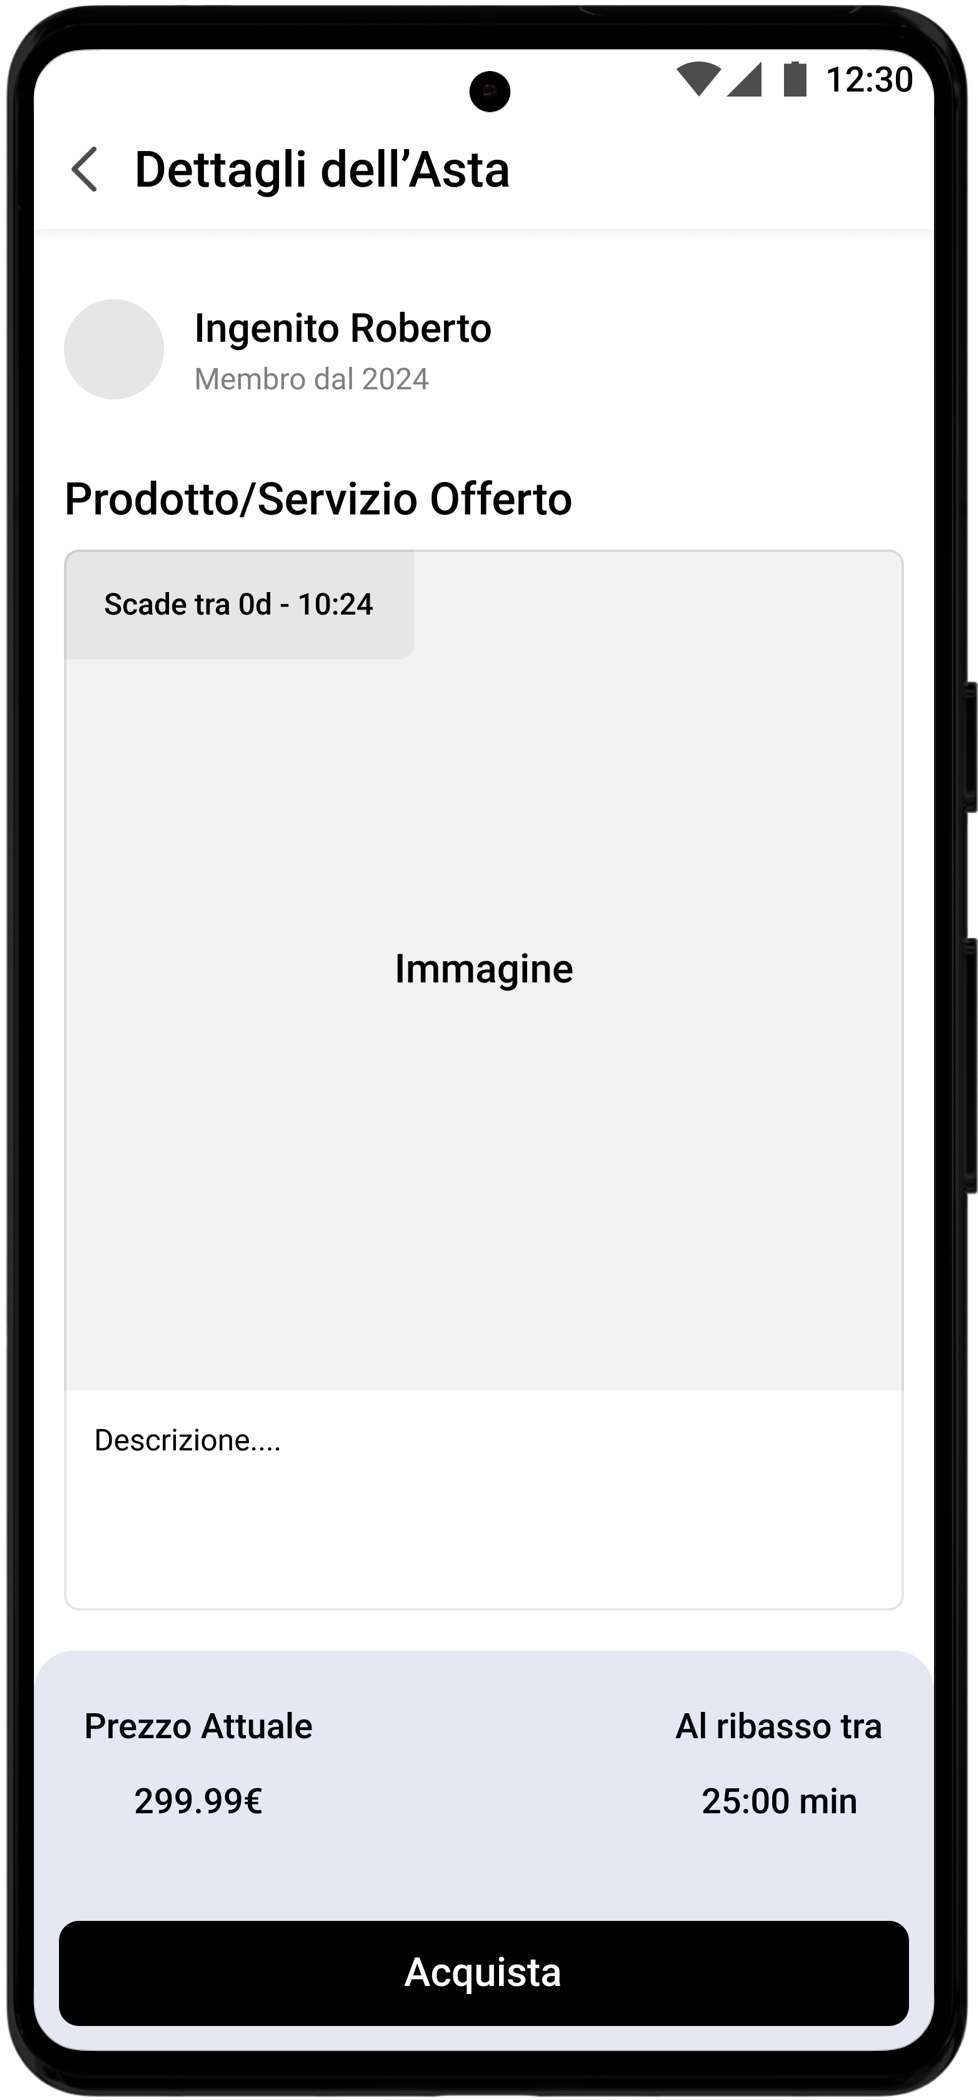
\includegraphics[width=.3\textwidth]{assets/mockup/Dettaglio Asta al Ribasso.png}  &
		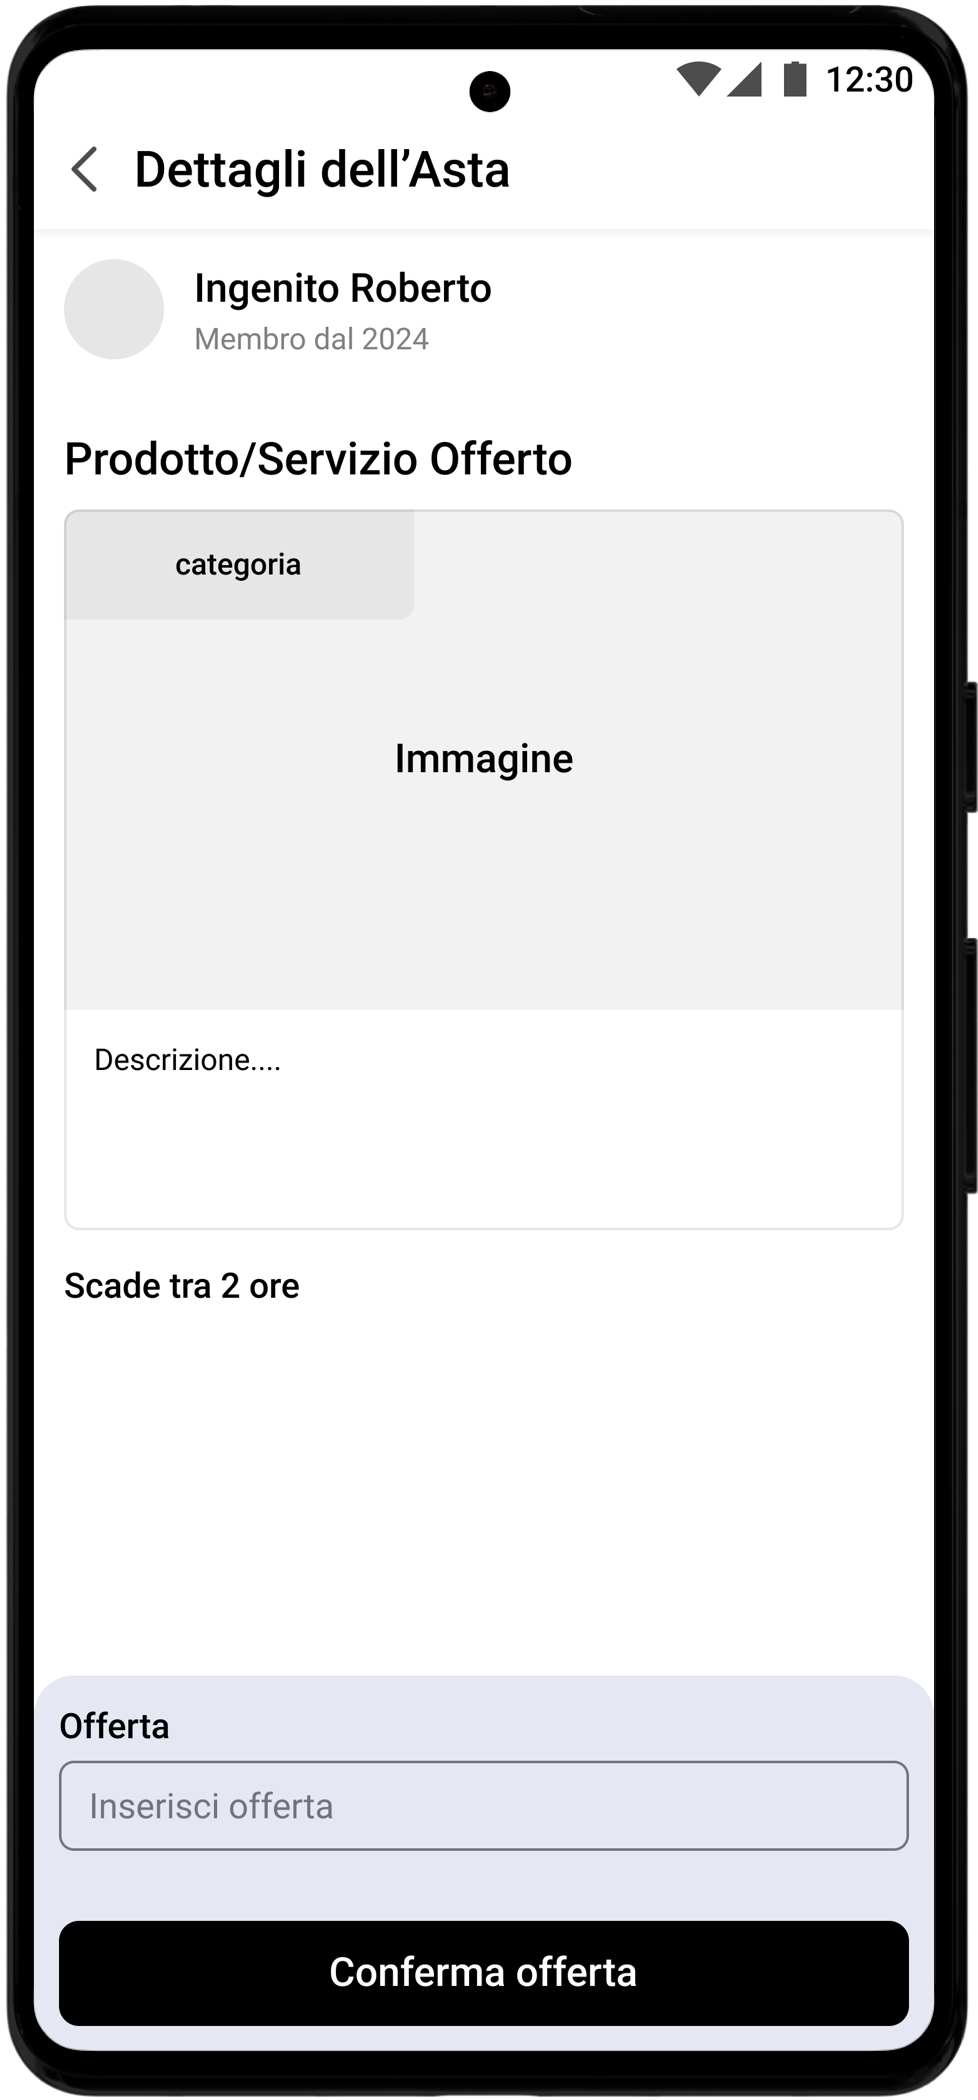
\includegraphics[width=.3\textwidth]{assets/mockup/Dettaglio Asta Silenziosa.png}    \\
	\end{tabular}
\end{center}

\newpage
\subsection{Creare un'asta}
Il primo mockup mostra la pagina dov'è possibile selezionare il tipo di asta che si vuole andare a creare.\\
Premendo sul pulsante "i" in alto a destra, apparirà la finestra mostrata nel secondo mockup dove vengono spiegate le differenze fra i tre tipi d'asta.\meskip
I tre mockup in basso, mostrano le pagine dei diversi tipi di creazione di un'asta.

\begin{center}
	\begin{tabular}{ccc}
		Seleziona tipo di asta                                           &  &
		Informazioni tipi d'asta                                                        \\
		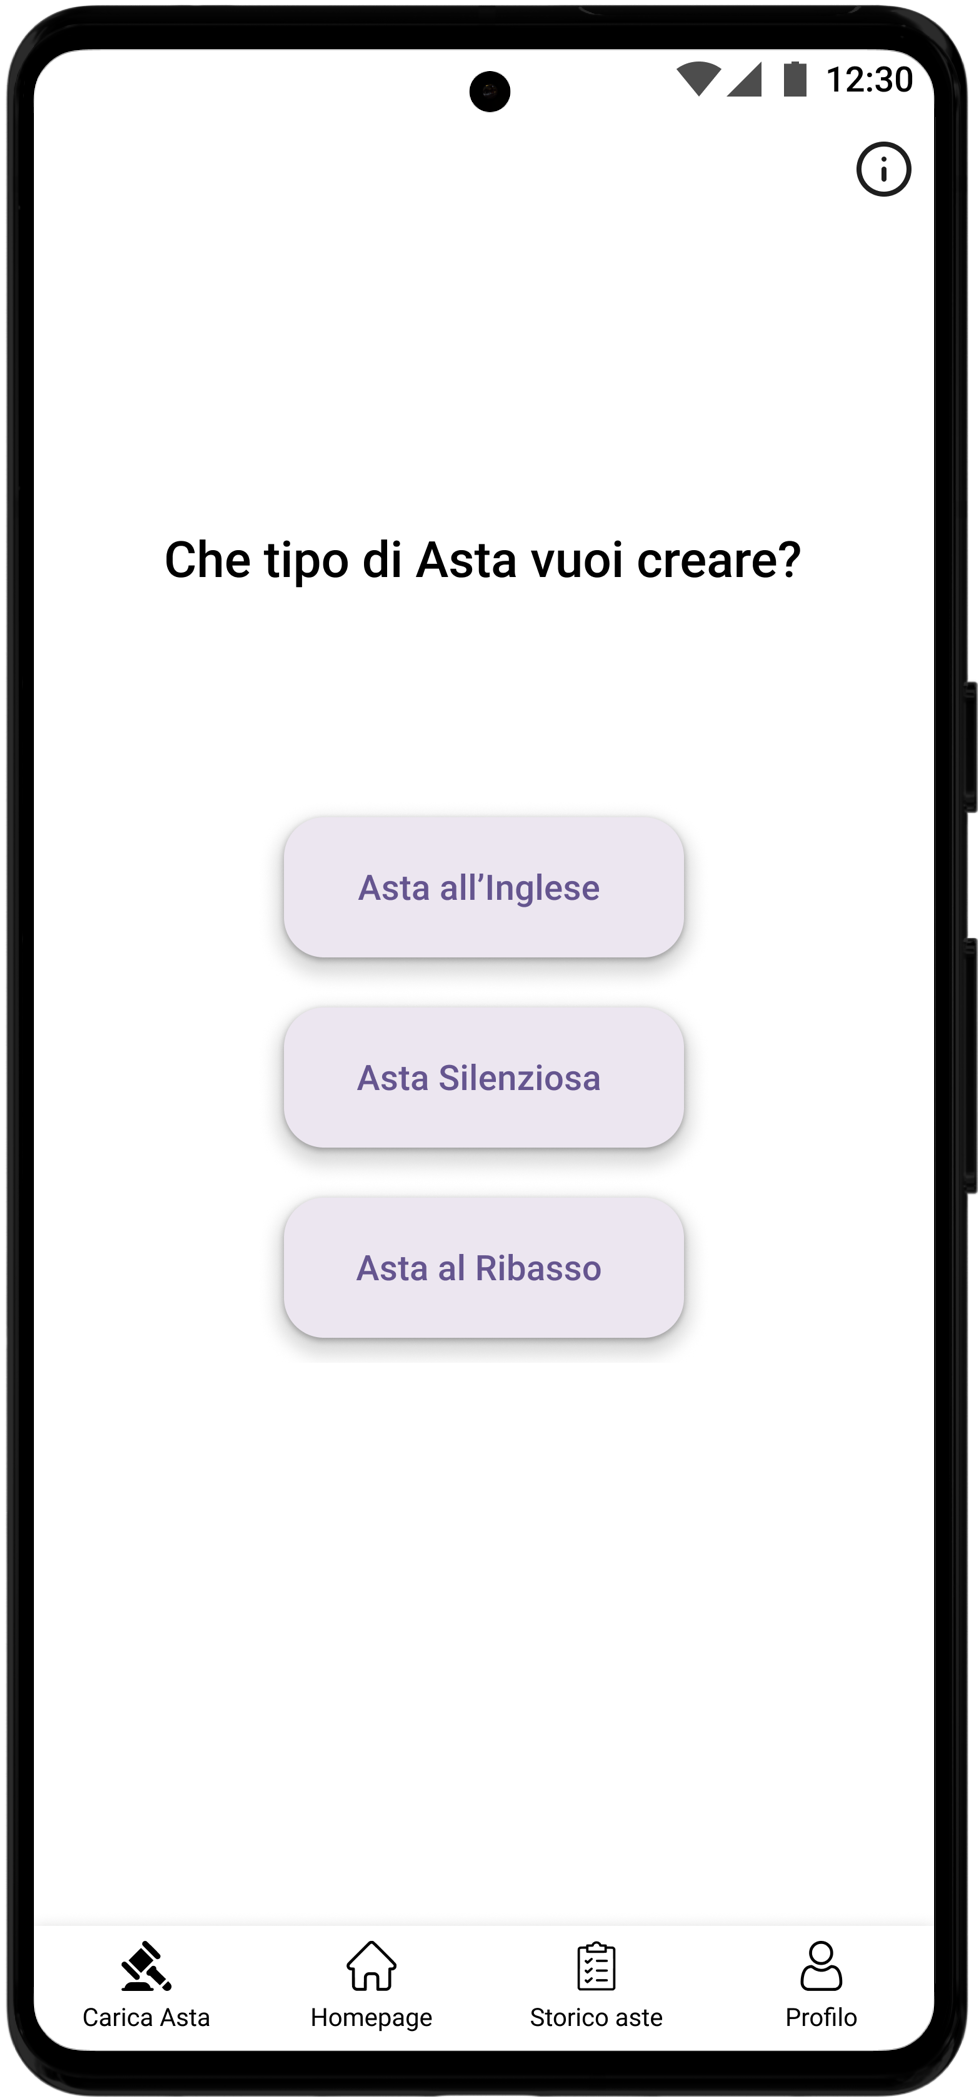
\includegraphics[height=280pt]{assets/mockup/Carica Asta 1..png} &  &
		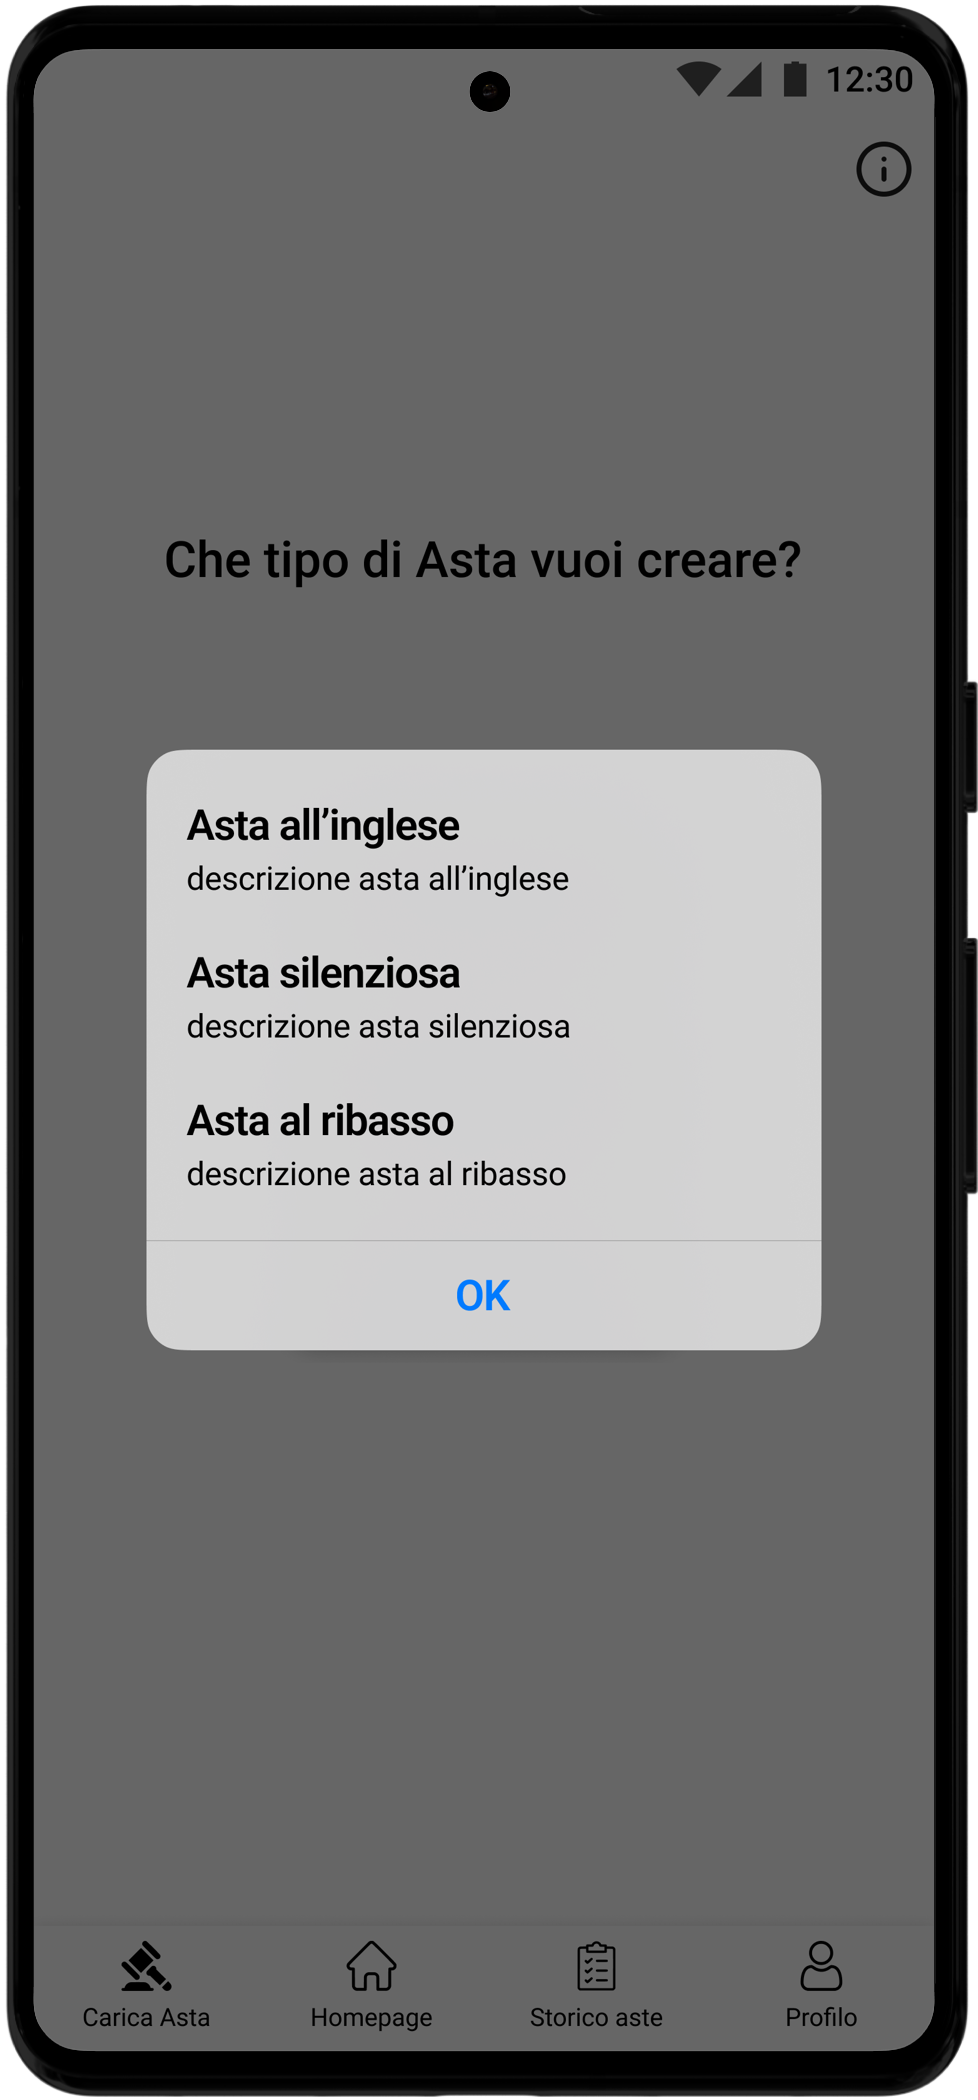
\includegraphics[height=280pt]{assets/mockup/Carica Asta 1. - informazioni.png} \\
	\end{tabular}
\end{center}
\begin{center}
	\begin{tabular}{ccccc}
		Creazione asta all'Inglese                                                         &  &
		Creazione asta al Ribasso                                                          &  &
		Creazione asta Silenziosa                                                               \\
		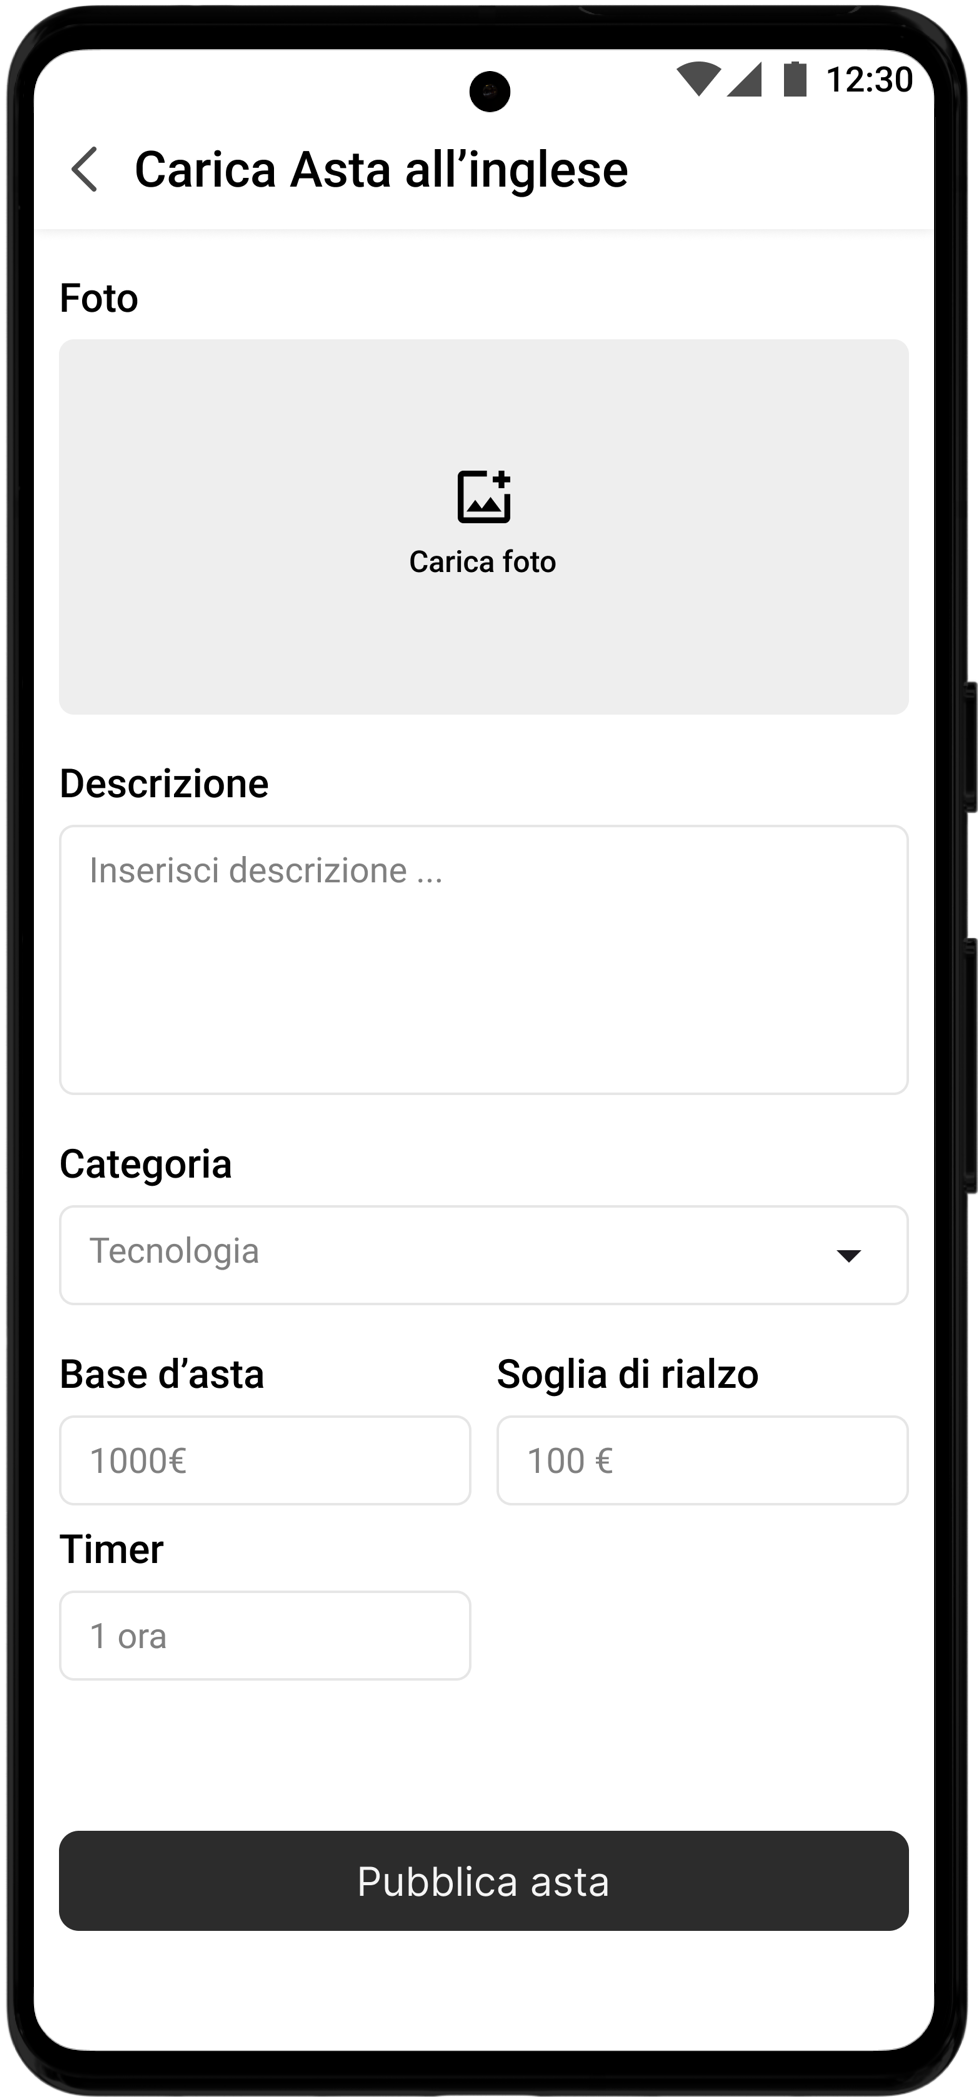
\includegraphics[height=280pt]{assets/mockup/Carica Asta 1.1 Asta all'Inglese.png} &  &
		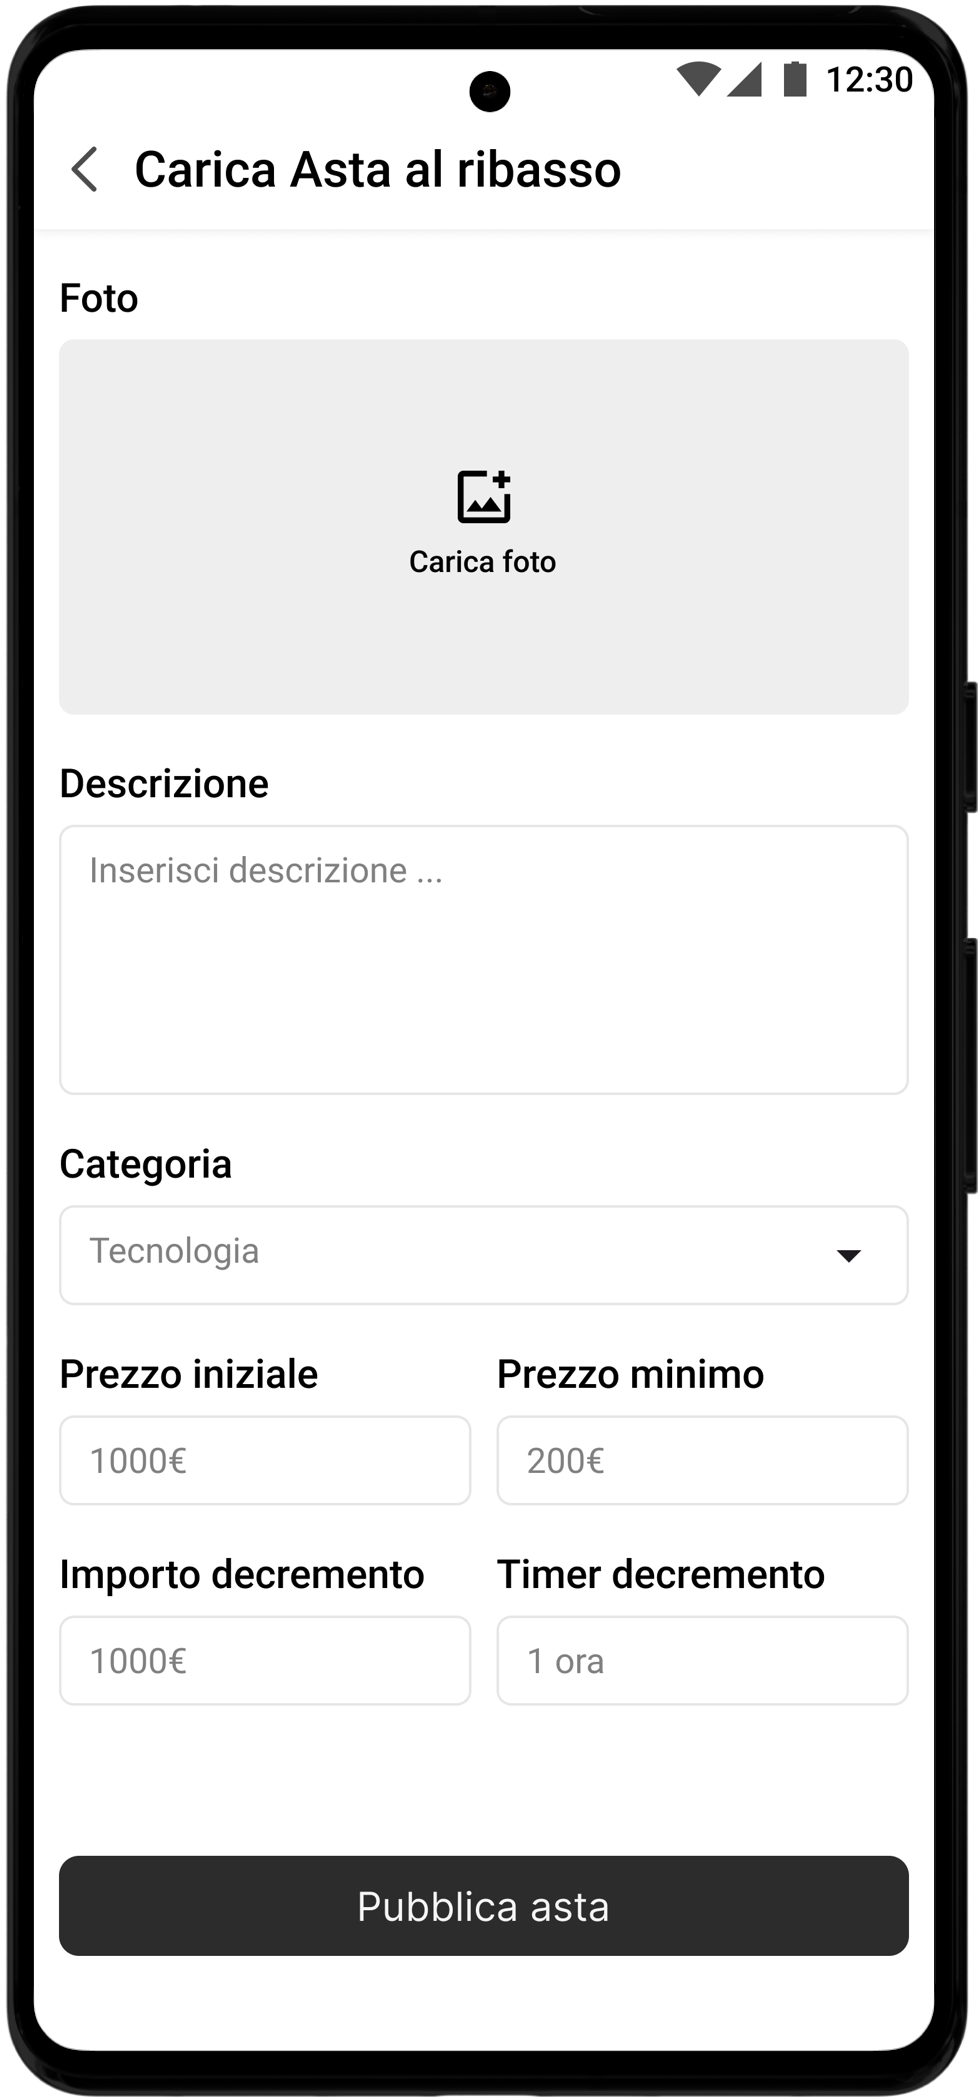
\includegraphics[height=280pt]{assets/mockup/Carica Asta 1.1 Asta al Ribasso.png}  &  &
		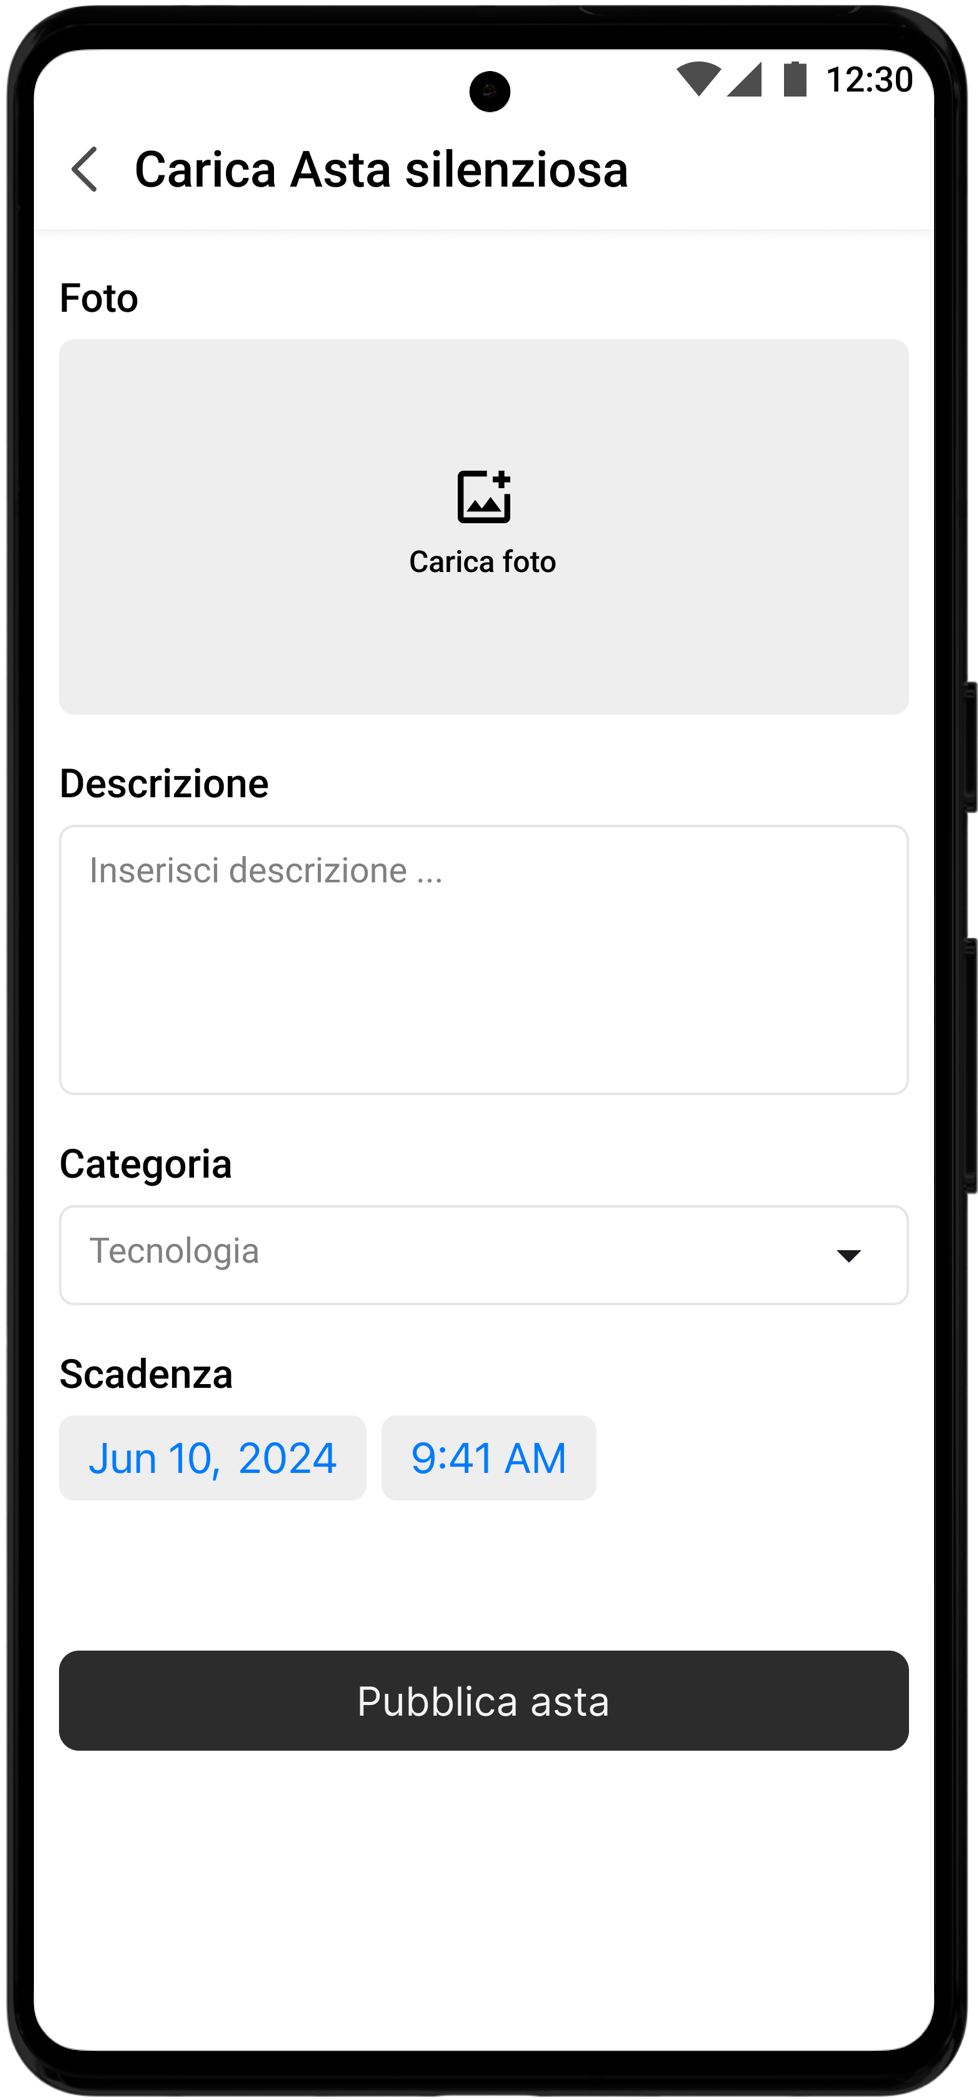
\includegraphics[height=280pt]{assets/mockup/Carica Asta 1.1 Asta Silenziosa.png}       \\
	\end{tabular}
\end{center}





\newpage

\section{Individuazione del target degli utenti.}
L'identificazione del target degli utenti è cruciale per garantire che l'applicazione soddisfi le esigenze e le aspettative dei suoi utilizzatori.

\subsection*{Descrizione del Servizio}
DietiDeals24 è un'applicazione progettata per facilitare la compravendita di beni e servizi tramite aste online.
Grazie a questa piattaforma, gli utenti possono partecipare a aste in tempo reale e avere l'opportunità di acquistare prodotti e servizi a prezzi vantaggiosi.\sskip
Di fatto l'applicazione si configura all'interno del settore e-commerce e questo ci ha permesso di fare analisi sul target degli utenti.

\subsection*{Target Demografici}
\begin{itemize}
	\item \textbf{Età}:
	      Il target principale si colloca nella fascia d'età tra 25 e 45 anni, che rappresenta una parte significativa degli acquirenti online, in particolare quelli che partecipano a piattaforme di e-commerce e aste online.
	\item \textbf{Genere}:
	      Tendenzialmente bilanciato, con una leggera prevalenza maschile nelle aste online, ma con un interesse crescente anche tra le donne.
	\item \textbf{Reddito}:
	      Medio, con utenti che cercano offerte vantaggiose ma che dispongono di un potere d'acquisto tale da consentire la partecipazione a aste su prodotti di valore medio-alto.
\end{itemize}

\subsection*{Target Geografici}
Utenti che vivono in città e usano spesso Internet per fare acquisti online.
Questi servizi sono più diffusi nelle zone dove la connessione è buona e la maggior parte delle persone sa usare bene la tecnologia.

\subsection*{Target Comportamentali}
Gli utenti che acquistano online tramite un servizio di aste solitamente cercano i seguenti benefici:
\begin{itemize}
	\item \textbf{Risparmio}: acquistare prodotti a prezzi più bassi grazie alla natura competitiva delle aste.
	\item \textbf{Prodotti esclusivi}: Possibilità di accedere a beni rari o di valore, che potrebbero non essere facilmente disponibili nei negozi tradizionali.
	\item \textbf{Soddisfazione della vittoria}: Vincere un'asta può essere un'esperienza gratificante e motivante.
\end{itemize}

\subsection*{Fonti}
Statista, "E-commerce user demographics in 2023", disponibile su \url{www.statista.com} .\\
Digital Commerce 360, "Who shops online?" disponibile su \url{www.digitalcommerce360.com} .

\section{Valutazione dell'usabilità a priori}
\subsection{Euristiche di Nielsen}
\begin{enumerate}
	\item \textbf{\sffamily Visibilità dello stato del sistema} \\
	      L'applicazione dovrebbe sempre tenere gli utenti informati su cosa sta succedendo, fornendo dei feedback immediati a seguito di un'azione.

	      Ad esempio, quando un utente effettua un'offerta, il sistema deve fornire un messaggio di conferma.

	\item \textbf{\sffamily Corrispondenza tra il sistema e il mondo reale} \\
	      L'applicazione dovrebbe utilizzare un linguaggio semplice, con termini che gli utenti comprendono facilmente, evitando il termini tecnici.
	      Ad esempio, i termini usati per descrivere le azioni come "Conferma offerta", "Modifica profilo"; oppure i messaggi di conferma come "Offerta confermata"/"Offerta rifiutata"

	\item \textbf{\sffamily Controllo dell'utente e libertà} \\
	      Gli utenti spesso commettono errori e dovrebbero essere in grado di annullare facilmente le azioni indesiderate.

	\item \textbf{\sffamily Coerenza e standard} \\
	      L'interfaccia dell'applicazione dovrebbe essere coerente in tutte le sue sezioni, sia in termini di design che di funzionalità.
	      Ad esempio i pulsanti, i colori e le azioni devono avere lo stesso significato in tutte le schermate.

	\item \textbf{\sffamily Prevenzione degli errori} \\
	      L'app dovrebbe prevenire gli errori rendendo difficile per gli utenti fare scelte sbagliate. È meglio progettare l'interfaccia in modo da evitare che gli errori accadano, piuttosto che fornire messaggi di errore.

	\item \textbf{\sffamily Riconoscimento piuttosto che ricordo} \\
	      Ridurre al minimo la quantità di informazioni che l'utente deve ricordare durante la navigazione.
	      Ad esempio, fornendo suggerimenti durante l'uso dell'app per agevolare l'interazione dell'utente.

	\item \textbf{\sffamily Flessibilità ed Efficienza} \\
	      L'app dovrebbe essere utilizzabile sia da utenti principianti che esperti.

	\item \textbf{\sffamily Design Estetico e Minimalista} \\
	      Le informazioni e le opzioni inutili dovrebbero essere eliminate.
	      Ogni elemento dell'interfaccia dovrebbe avere uno scopo chiaro.

	\item \textbf{\sffamily Aiuto e Documentazione} \\
	      L'applicazione dovrebbe essere facile da usare senza documentazione, dovrebbe esserci comunque un aiuto disponibile per gli utenti che lo richiedono.

	\item \textbf{\sffamily Gestione degli Errori} \\
	      Se si verificano errori, il sistema dovrebbe presentare messaggi d'errore chiari e non codici d'errore.
\end{enumerate}

\section{Specifica dei requisiti}
\subsection{Modelli di dominio}
\subsection*{Registrazione e accesso}
\begin{center}
	\scalebox{0.7}{
		\begin{tikzpicture}
			\umlclass[x=0, y=0, type=Boundary]{SignUpForm}{
				+ firstName: TextField\\
				+ lastName: TextField\\
				+ email: TextField\\
				+ password: TextField\\
				+ goToSignInPage: Button\\
				+ signUp: Button\\
			}{}

			\umlclass[x=10, y=0, type=Boundary]{SignInForm}{
				+ email: TextField\\
				+ password: TextField\\
				+ signIn: Button\\
				+ goToSignUpPage: Button\\
				+ signInWithGoogle: Button\\
			}{}
			\umlclass[x=5, y=-5, type=Boundary]{Feedback}{
				+ message: String \\
			}{}
			\umlclass[x=0, y=-9, type=Control]{SignUpController}{}{
				+ signUp(firstName, lastName, email, password)
			}
			\umlclass[x=10, y=-9, type=Control]{SignInController}{}{
				+ signIn(email, password)\\
				+ signInWithGoogle()
			}
			\umlclass[x=5, y=-15, type=Entity]{User}{
				+ firstName: String \\
				+ lastName: String \\
				+ email: String \\
				+ password: String \\
				+ bio: String \\
				+ webSiteLink: String \\
				+ profileImagePath: String \\
				+ socialLink: String[] \\
			}{}

			% Relationships
			\umlassoc[line width=2pt]{SignUpForm}{SignInForm}
			\umlassoc[line width=2pt]{SignUpForm}{SignUpController}
			\umlassoc[line width=2pt]{SignInForm}{SignInController}
			\umlassoc[line width=2pt]{SignUpController}{User}
			\umlassoc[line width=2pt]{SignInController}{User}
			\umlassoc[line width=2pt]{SignUpController}{Feedback}
			\umlassoc[line width=2pt]{SignInController}{Feedback}
		\end{tikzpicture}
	}
\end{center}

\newpage
\subsection*{Creazione asta silenziosa}
\begin{center}
	\scalebox{0.7}{
		\begin{tikzpicture}
			\umlclass[type=Boundary, x=9, y=-4]{CreateAuction}{
				+ descendingAuctionButton: Button \\
				+ englishAuctionButton: Button \\
				+ silentAuctionButton: Button \\
			}{}

			\umlclass[type=Boundary, left=3cm of CreateAuction, yshift=1.5cm]{CreateDescendingAuction}{
			}{}

			\umlclass[type=Boundary, left=3cm of CreateAuction, yshift=-1.5cm]{CreateEnglishAuction}{
			}{}

			\umlclass[type=Boundary, right=3cm of CreateAuction, yshift=1cm]{NavBar}{
				+ createAuctionButton: Button
			}{}

			\umlclass[type=Boundary, below=1cm of CreateAuction]{CreateSilentAuction}{
				+ loadImageButton: Button \\
				+ descriptionTextField: TextField \\
				+ categorySelect: Select \\
				+ dateTimePicker: DateTimePicker \\
				+ publishButton: Button \\
			}{}

			\umlclass[type=Control, below=1cm of CreateSilentAuction]{CreateAuctionController}{}{
				+ createSilentAuction(image, description, category, expirationDateTime) \\
				+ createDescendingAuction() \\
				+ createEnglishAuction()
			}

			\umlclass[type=Boundary, right=1cm of CreateAuctionController, yshift=4cm]{Feedback}{
				+ message: String
			}{}

			\umlclass[type=Entity, x=1, y=-19]{DescendingAuction}{
			}{}
			\umlclass[type=Entity, x=0, y=-22]{EnglishAuction}{
			}{}
			\umlclass[type=Entity, below=1cm of CreateAuctionController]{SilentAuction}{
				+ expirationDateTime: DateTime \\
			}{}

			\umlclass[type=Entity, below=1cm of SilentAuction]{Auction}{
				+ description: String \\
				+ imagePath: String \\
				+ category: String \\
			}{}

			\umlclass[below=1.5cm of Auction, type=Entity]{User}{
				+ firstName: String \\
				+ lastName: String \\
				+ email: String \\
				+ password: String \\
				+ bio: String \\
				+ webSiteLink: String \\
				+ profileImagePath: String \\
				+ socialLink: String[] \\
			}{}

			% Relationships
			\umlassoc{CreateAuction}{CreateDescendingAuction}
			\umlassoc{CreateAuction}{CreateEnglishAuction}
			\umlassoc{CreateAuction}{NavBar}
			\umlassoc{CreateAuction}{CreateSilentAuction}
			\umlassoc{CreateSilentAuction}{CreateAuctionController}
			\umlassoc{CreateAuctionController}{Feedback}
			\umlassoc{CreateAuctionController}{SilentAuction}
			\umlinherit{SilentAuction}{Auction}
			\umlinherit{EnglishAuction}{Auction}
			\umlinherit{DescendingAuction}{Auction}
			\umlassoc[mult2=1, mult1=0..*]{Auction}{User}
		\end{tikzpicture}
	}
\end{center}

\newpage
\subsection*{Creazione asta all'inglese}
\begin{center}
	\scalebox{0.7}{
		\begin{tikzpicture}
			\umlclass[type=Boundary, x=9, y=-4]{CreateAuction}{
				+ descendingAuctionButton: Button \\
				+ englishAuctionButton: Button \\
				+ silentAuctionButton: Button \\
			}{}

			\umlclass[type=Boundary, left=3cm of CreateAuction, yshift=1.5cm]{CreateDescendingAuction}{
			}{}

			\umlclass[type=Boundary, left=3cm of CreateAuction, yshift=-1.5cm]{CreateSilentAuction}{
			}{}

			\umlclass[type=Boundary, right=3cm of CreateAuction, yshift=1cm]{NavBar}{
				+ createAuctionButton: Button
			}{}

			\umlclass[type=Boundary, below=1cm of CreateAuction]{CreateEnglishAuction}{
				+ loadImageButton: Button \\
				+ descriptionTextField: TextField \\
				+ categorySelect: Select \\
				+ startingPriceTextField: TextField \\
				+ increaseThresholdTextField: TextField \\
				+ timerTextField: TextField \\
				+ publishButton: Button \\
			}{}

			\umlclass[type=Control, below=1cm of CreateEnglishAuction]{CreateAuctionController}{}{
				+ createEnglishAuction(image, description, category, startingPrice, increaseThreshold, timer) \\
				+ createDescendingAuction() \\
				+ createSilentAuction()
			}

			\umlclass[type=Boundary, right=1cm of CreateAuctionController, yshift=4cm]{Feedback}{
				+ message: String
			}{}

			\umlclass[type=Entity, below=1cm of CreateAuctionController]{EnglishAuction}{
				+ startingPrice: double \\
				+ increaseThreshold: double \\
				+ timer: int \\
			}{}

			\umlclass[type=Entity, below=1cm of EnglishAuction]{Auction}{
				+ description: String \\
				+ imagePath: String \\
				+ category: String \\
			}{}

			\umlclass[type=Entity, left=3cm of Auction, yshift=4cm]{DescendingAuction}{
			}{}
			\umlclass[type=Entity, left=5cm of Auction, yshift=1cm]{SilentAuction}{
			}{}

			\umlclass[below=1.5cm of Auction, type=Entity]{User}{
				+ firstName: String \\
				+ lastName: String \\
				+ email: String \\
				+ password: String \\
				+ bio: String \\
				+ webSiteLink: String \\
				+ profileImagePath: String \\
				+ socialLink: String[] \\
			}{}

			% Relationships
			\umlassoc{CreateAuction}{CreateDescendingAuction}
			\umlassoc{CreateAuction}{CreateSilentAuction}
			\umlassoc{CreateAuction}{NavBar}
			\umlassoc{CreateAuction}{CreateEnglishAuction}
			\umlassoc{CreateEnglishAuction}{CreateAuctionController}
			\umlassoc{CreateAuctionController}{Feedback}
			\umlassoc{CreateAuctionController}{EnglishAuction}
			\umlinherit{SilentAuction}{Auction}
			\umlinherit{EnglishAuction}{Auction}
			\umlinherit{DescendingAuction}{Auction}
			\umlassoc[mult2=1, mult1=0..*]{Auction}{User}
		\end{tikzpicture}
	}
\end{center}

\newpage
\subsection*{Creazione asta al ribasso}
\begin{center}
	\scalebox{0.67}{
		\begin{tikzpicture}
			\umlclass[type=Boundary, x=9, y=0]{AuctionTypeCreationPage}{
				+ descendingAuctionButton: Button \\
				+ englishAuctionButton: Button \\
				+ silentAuctionButton: Button \\
			}{}

			\umlclass[type=Boundary, left=3cm of AuctionTypeCreationPage, yshift=1.5cm]{CreateEnglishAuction}{
			}{}
			
			\umlclass[type=Boundary, left=3cm of AuctionTypeCreationPage, yshift=-1.5cm]{CreateSilentAuction}{
			}{}

			\umlclass[type=Boundary, right=3cm of AuctionTypeCreationPage, yshift=1cm]{NavBar}{
				+ createAuctionButton: Button
			}{}

			\umlclass[type=Boundary, below=1cm of AuctionTypeCreationPage]{CreateDescendingAuction}{
				+ loadImageButton: Button \\
				+ descriptionTextField: TextField \\
				+ categorySelect: Select \\
				+ startingPriceTextField: TextField \\
				+ minimumPriceTextField: TextField \\
				+ decreaseAmountTextField: TextField \\
				+ decreaseTimeTextField: TextField \\
				+ publishButton: Button \\
			}{}

			\umlclass[type=Control, below=1cm of CreateDescendingAuction]{CreateAuctionController}{}{
				+ createDescendingAuction( image, description, category, \\
				\hspace{5cm}startingPrice, minimumPrice, \\
				\hspace{5cm}decreaseAmount, decreaseTime ) \\
				+ createEnglishAuction() \\
				+ createSilentAuction()
			}

			\umlclass[type=Boundary, right=1cm of CreateAuctionController, yshift=4cm]{Feedback}{
				+ message: String
			}{}

			\umlclass[type=Entity, below=1cm of CreateAuctionController]{DescendingAuction}{
				+ startingPrice: double \\
				+ minimumPrice: double \\
				+ decreaseAmount: double \\
				+ decreaseTime: int \\
			}{}

			\umlclass[type=Entity, below=1cm of DescendingAuction]{Auction}{
				+ description: String \\
				+ imagePath: String \\
				+ category: String \\
			}{}
			
			\umlclass[type=Entity, left=3cm of Auction, yshift=4cm]{EnglishAuction}{
			}{}
			\umlclass[type=Entity, left=5cm of Auction, yshift=1cm]{SilentAuction}{
			}{}

			\umlclass[below=1.5cm of Auction, type=Entity]{User}{
				+ firstName: String \\
				+ lastName: String \\
				+ email: String \\
				+ password: String \\
				+ bio: String \\
				+ webSiteLink: String \\
				+ profileImagePath: String \\
				+ socialLink: String[] \\
			}{}
			
			% Relationships
			\umlassoc{AuctionTypeCreationPage}{CreateEnglishAuction}
			\umlassoc{AuctionTypeCreationPage}{CreateSilentAuction}
			\umlassoc{AuctionTypeCreationPage}{NavBar}
			\umlassoc{AuctionTypeCreationPage}{CreateDescendingAuction}
			\umlassoc{CreateDescendingAuction}{CreateAuctionController}
			\umlassoc{CreateAuctionController}{Feedback}
			\umlassoc{CreateAuctionController}{DescendingAuction}
			\umlinherit{SilentAuction}{Auction}
			\umlinherit{DescendingAuction}{Auction}
			\umlinherit{EnglishAuction}{Auction}
			\umlassoc[mult2=1, mult1=0..*]{Auction}{User}
		\end{tikzpicture}
	}
\end{center}


\newpage
